% Тип документа
\documentclass[a4paper,12pt]{extarticle}

% Шрифты, кодировки, символьные таблицы, переносы
\usepackage{cmap}
\usepackage[T2A]{fontenc}
\usepackage[utf8x]{inputenc}
\usepackage[russian]{babel}

% Это пакет -- хитрый пакет, он нужен но не нужен
\usepackage[mode=buildnew]{standalone}

\usepackage
	{
		% Дополнения Американского математического общества (AMS)
		amssymb,
		amsfonts,
		amsmath,
		amsthm,
		physics,
		% misccorr,
		% 
		% Графики и рисунки
		wrapfig,
		graphicx,
		subcaption,
		float,
		tikz,
		tikz-3dplot,
		caption,
		csvsimple,
		color,
		booktabs,
		pgfplots,
		pgfplotstable,
		geometry,
		% 
		% Таблицы, списки
		makecell,
		multirow,
		indentfirst,
		%
		% Интегралы и прочие обозначения
		ulem,
		esint,
		esdiff,
		% 
		% Колонтитулы
		fancyhdr,
	}  

\usepackage{xcolor}
\usepackage{hyperref}

 % Цвета для гиперссылок
\definecolor{linkcolor}{HTML}{000000} % цвет ссылок
\definecolor{urlcolor}{HTML}{799B03} % цвет гиперссылок
 
\hypersetup{pdfstartview=FitH,  linkcolor=linkcolor,urlcolor=urlcolor, colorlinks=true}
% Обводка текста в TikZ
\usepackage[outline]{contour}

% Увеличенный межстрочный интервал, французские пробелы
\linespread{1.3} 
\frenchspacing 

 
\usetikzlibrary
	{
		decorations.pathreplacing,
		decorations.pathmorphing,
		patterns,
		calc,
		scopes,
		arrows,
		fadings,
		through,
		shapes.misc,
		arrows.meta,
		3d,
		quotes,
		angles,
		babel
	}


\tikzset{
	force/.style=	{
		>=latex,
		draw=blue,
		fill=blue,
				 	}, 
	%				 	
	axis/.style=	{
		densely dashed,
		blue,
		line width=1pt,
		font=\small,
					},
	%
	th/.style=	{
		line width=1pt},
	%
	acceleration/.style={
		>=open triangle 60,
		draw=magenta,
		fill=magenta,
					},
	%
	inforce/.style=	{
		force,
		double equal sign distance=2pt,
					},
	%
	interface/.style={
		pattern = north east lines, 
		draw    = none, 
		pattern color=gray!60,
					},
	cross/.style=	{
		cross out, 
		draw=black, 
		minimum size=2*(#1-\pgflinewidth), 
		inner sep=0pt, outer sep=0pt,
					},
	%
	cargo/.style=	{
		rectangle, 
		fill=black!70, 
		inner sep=2.5mm,
					},
	%
	caption/.style= {
		midway,
		fill=white!20, 
		opacity=0.9
					},
	%
	}

\newenvironment{tikzpict}
    {
	    \begin{figure}[htbp]
		\centering
		\begin{tikzpicture}
    }
    { 
		\end{tikzpicture}
		% \caption{caption}
		% \label{fig:label}
		\end{figure}
    }


\newcommand{\vbLabel}[3]{\draw ($(#1,#2)+(0,5pt)$) -- ($(#1,#2)-(0,5pt)$) node[below]{#3}}
\newcommand{\vaLabel}[3]{\draw ($(#1,#2)+(0,5pt)$) node[above]{#3} -- ($(#1,#2)-(0,5pt)$) }

\newcommand{\hrLabel}[3]{\draw ($(#1,#2)+(5pt,0)$) -- ($(#1,#2)-(5pt,0)$) node[right, xshift=1em]{#3}}
\newcommand{\hlLabel}[3]{\draw ($(#1,#2)+(5pt,0)$) node[left, xshift=-1em]{#3} -- ($(#1,#2)-(5pt,0)$) }



\newcommand\zi{^{\,*}_i}
\newcommand\sumn{\sum_{i=1}^{N}}

\tikzset{
	coordsys/.style={scale=1.8,x={(1.1cm,-0cm)},y={(0.5cm,1cm)}, z={(0cm,0.8cm)}},
	coordsys/.style={scale=1.5,x={(0cm,0cm)},y={(1cm,0cm)}, z={(0cm,1cm)}}, 
	coordsys/.style={scale=1.5,x={(1cm,0cm)},y={(0cm,1cm)}, z={(0cm,0cm)}}, 
}

\usepgfplotslibrary{units}


% Draw line annotation
% Input:
%   #1 Line offset (optional)
%   #2 Line angle
%   #3 Line length
%   #5 Line label
% Example:
%   \lineann[1]{30}{2}{$L_1$}

\newcommand{\lineann}[4][0.5]{%
    \begin{scope}[rotate=#2, blue,inner sep=2pt, ]
        \draw[dashed, blue!40] (0,0) -- +(0,#1)
            node [coordinate, near end] (a) {};
        \draw[dashed, blue!40] (#3,0) -- +(0,#1)
            node [coordinate, near end] (b) {};
        \draw[|<->|] (a) -- node[fill=white, scale=0.8] {#4} (b);
    \end{scope}
}

\newcommand{\lineannn}[4][0.5]{%
    \begin{scope}[rotate=#2, blue,inner sep=2pt, ]
        \draw[dashed, blue!40] (0,0) -- +(0,#1)
            node [coordinate, near end] (a) {};
        \draw[dashed, blue!40] (#3,0) -- +(0,#1)
            node [coordinate, near end] (b) {};
        % \draw[color=white, color=blue] (a) -- node[fill=white, scale=0.8] {#4} (b);
        \draw[->|] (a)++(-0.3,0) -- (a);
        \draw[->|] (b)++(0.3,0) coordinate (xx) -- (b);
        \draw (xx) node[fill=white, scale=0.8, right] {#4};
    \end{scope}
}

% Круговая стрелка относительно центра (дуга из центра)
\tikzset{
  pics/carc/.style args={#1:#2:#3}{
    code={
      \draw[pic actions] (#1:#3) arc(#1:#2:#3);
    }
  },
  dash/.style={
  	dash pattern=on 5mm off 5mm
  }
}

% Среднее <#1>
\newcommand{\mean}[1]{\langle#1\rangle}

\pgfplotsset{
    % most recent feature set of pgfplots
    compat=newest,
}

% const прямым шрифтом
\newcommand\ct[1]{\text{\rmfamily\upshape #1}}
\newcommand*{\const}{\ct{const}}


\usepackage[europeanresistors,americaninductors]{circuitikz}

% Style to select only points from #1 to #2 (inclusive)
\pgfplotsset{select/.style 2 args={
    x filter/.code={
        \ifnum\coordindex<#1\def\pgfmathresult{}\fi
        \ifnum\coordindex>#2\def\pgfmathresult{}\fi
    }
}}


\usepackage{array}
\usepackage{pstool}


%%%%%%%%%%%%%%%%%%%%%%%%%%%%%%%%%%%%%%%%%%%%%%%%%
\makeatletter
\newif\if@gather@prefix 
\preto\place@tag@gather{% 
  \if@gather@prefix\iftagsleft@ 
    \kern-\gdisplaywidth@ 
    \rlap{\gather@prefix}% 
    \kern\gdisplaywidth@ 
  \fi\fi 
} 
\appto\place@tag@gather{% 
  \if@gather@prefix\iftagsleft@\else 
    \kern-\displaywidth 
    \rlap{\gather@prefix}% 
    \kern\displaywidth 
  \fi\fi 
  \global\@gather@prefixfalse 
} 
\preto\place@tag{% 
  \if@gather@prefix\iftagsleft@ 
    \kern-\gdisplaywidth@ 
    \rlap{\gather@prefix}% 
    \kern\displaywidth@ 
  \fi\fi 
} 
\appto\place@tag{% 
  \if@gather@prefix\iftagsleft@\else 
    \kern-\displaywidth 
    \rlap{\gather@prefix}% 
    \kern\displaywidth 
  \fi\fi 
  \global\@gather@prefixfalse 
} 
\newcommand*{\beforetext}[1]{% 
  \ifmeasuring@\else
  \gdef\gather@prefix{#1}% 
  \global\@gather@prefixtrue 
  \fi
} 
\makeatother
%%%%%%%%%%%%%%%%%%%%%%%%%%%%%%%%%%%%%%%%%%%%%%%%%

\geometry		
	{
		left			=	2cm,
		right 			=	2cm,
		top 			=	3cm,
		bottom 			=	3cm,
		bindingoffset	=	0cm
	}

%%%%%%%%%%%%%%%%%%%%%%%%%%%%%%%%%%%%%%%%%%%%%%%%%%%%%%%%%%%%%%%%%%%%%%%%%%%%%%%



	%применим колонтитул к стилю страницы
\pagestyle{fancy} 
	%очистим "шапку" страницы
\fancyhead{} 
	%слева сверху на четных и справа на нечетных
\fancyhead[R]{\labauthors} 
	%справа сверху на четных и слева на нечетных
\fancyhead[L]{Отчёт по лабораторной работе №\labnumber} 
	%очистим "подвал" страницы
\fancyfoot{} 
	% номер страницы в нижнем колинтуле в центре
\fancyfoot[C]{\thepage} 

%%%%%%%%%%%%%%%%%%%%%%%%%%%%%%%%%%%%%%%%%%%%%%%%%%%%%%%%%%%%%%%%%%%%%%%%%%%%%%%

\renewcommand{\contentsname}{Оглавление}

\usepackage{tocloft}
% \renewcommand{\cftpartleader}{\cftdotfill{\cftdotsep}} % for parts
% \renewcommand{\cftsectiondotsep}{\cftdotsep}% Chapters should use dots in ToC
\renewcommand{\cftsecleader}{\cftdotfill{\cftdotsep}}
%\renewcommand{\cftsecleader}{\cftdotfill{\cftdotsep}} % for sections, if you really want! (It is default in report and book class (So you may not need it).
% ---------
% \newcommand{\cftchapaftersnum}{.}%
% \usepackage{titlesec}
% \titlelabel{\thetitle.\quad}
\usepackage{secdot}
\sectiondot{subsection}
\usepackage{gensymb}
\usepackage{textcomp}
\usepackage{pythontex}

\begin{document}
\def\labauthors{Карусевич А.А, Понур К.А.}
\def\labgroup{430}
\def\department{Кафедра электродинамики}
\def\labnumber{1}
\def\labtheme{Исследование отражательного клистрона}

\renewcommand{\Re}{\operatorname{Re}}
\renewcommand{\Im}{\operatorname{Im}}
\renewcommand{\phi}{\varphi}
\renewcommand{\hat}{\widehat}

\begin{titlepage}

\begin{center}

{\small\textsc{Нижегородский государственный университет имени Н.\,И. Лобачевского}}
\vskip 1pt \hrule \vskip 3pt
{\small\textsc{Радиофизический факультет}}



\vfill
{\Large {\department}}

{\Large Отчет по лабораторной работе №\labnumber\vskip 12pt\bfseries \labtheme}
	
\end{center}

\vfill
	
\begin{flushright}
	{Выполнили студенты \labgroup\ группы\\ \labauthors}%\vskip 12pt Принял:\\ Менсов С.\,Н.}
\end{flushright}
	
\vfill
	
\begin{center}
	Нижний Новгород, \the\year
\end{center}

\end{titlepage}


\tableofcontents
%\newpage

\section{Теоретическая часть}

\addcontentsline{toc}{subsection}{Введение}
\subsection*{Введение}

Отражательный клистрон
\footnote{Название <<клистрон>> происходит от греческого слова «клизо», что означает береговой волнорез.}, 
изучению которого посвящена лабораторная работа, предназначен для генерации электромагнитных колебаний СВЧ диапазона. Исторически именно генераторы клистронного типа позволили освоить диапазоны сантиметровых и дециметровых волн, в которых традицион­ные электронные лампы оказались неэффективными [1].

Генерация в клистронах осуществляется за счет преобразования кинетической энергии пучка электронов, ускоренных статическим электрическим полем, в энергию сверхвысокочастотных колебаний. Для получения СВЧ колебаний пучок электронов модулируется по плотности и проводится че­ рез резонатор клистрона, в котором переменный конвекционный ток пучка возбуждает колебания.

Неоднородный электронный поток в приборах клистронного типа созда­ется посредством так называемого динамического способа управления плот­ностью зарядов. При этом способе управления однородный электронный по­ток пропускается через переменное электрическое поле управляющего 
(груп­пирующего) устройства. Переменное поле воздействует на скорости электро­
нов в потоке, периодически ускоряя и замедляя их движение в зависимо­
сти от фазы высокочастотного поля, существующей в момент пролета элек­тронов через управляющее устройство. Возникающее различие в скоростях
электронов приводит к их группировке при последующем движении за пре­
делами управляющего устройства. При этом в определенной точке простран­
ства в определенный момент времени происходит образование электронного
сгустка. Поток приобретает пульсирующий характер, причем электронные
уплотнения и разрежения в данной точке пространства возникают с перио­дичностью, соответствующей частоте управляющего поля
\footnote{При использовании приемов т. н. электростатического управления основной результат управ­
ления состоит в мо дуляции электронного потока по плотности непосредственно в области управ­
ляющего поля [2, 3].}.

Характер процесса группировки электронов, координата и время образования сгустка в клистронах определяются условиями движения вне управляющего промежутка.

В пролетных клистронах группировка происходит при движении электронов по инерции в пространстве, свободном от внешних постоянных или переменных полей; группировка становится возможной за счет того, что «быстрые» электроны догоняют «медленные», вылетевшие из управляюще­го промежутка раньше «быстрых».

В отражательных клистронах электроны, вышедшие из группирующего устройства, движутся в постоянном тормозящем электрическом поле. Значение этого поля таково, что все электроны, вылетевшие из управляющего устройства, возвращаются назад. Группировка в отражательных клистронах происходит благодаря тому, что «быстрые» электроны находятся в пространстве группировки дольше «медленных», и на обратном пути оказывается возможной встреча «быстрых» электронов с медленными, вышедшими из управляющего промежутка позже «быстрых».

Принципиальная схема отражательного клистрона представлена на рис. \ref{fig:1}. Функции управляющего устройства и устройства, накапливающего энергию электромагнитных колебаний в отражательном клистроне, объединены здесь в тороидальном резонаторе.

\begin{figure}[h!]
	\centering
	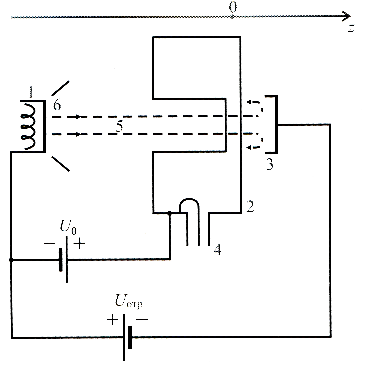
\includegraphics[width=0.4\textwidth]{fig/fig1}
	\caption{Идеализированная принципиальная схема клистрона: 1 — катод, 2 — резонатор, 3 — отражатель, 4 — вывод энергии, 5 — электронный поток, 6 — управляющий электрод}
	\label{fig:1}
\end{figure}

Электронный поток, эмитируемый катодом, ускоряется в промежутке между катодом и резонатором, после чего первый раз попадает в зазор резонатора, образованный двумя прозрачными для потока металлическими сетками. В зазоре происходит модуляция электронного потока по скорости. После выхода из резонатора электроны движутся в тормозящем поле отражающего электрода, возвращаются назад и повторно проходят зазор. При соответствующем выборе потенциалов на электродах клистрона сгусток электронов формируется в сечении зазора резонатора в момент времени, когда высокочастотное поле в зазоре тормозит возвращающиеся электроны, при этом происходит преобразование кинетической энергии электронов в энергию колебаний резонатора. Существование стационарных колебаний в клистроне оказывается возможным при компенсации потерь и резонаторе и нагрузке притоком энергии от модулированного электронного потока.

\subsection{Резонатор клистрона}

Резонатор в клистроне выполняет две функции: служит для модуляции электронного потока по скорости и для преобразования кинетической энергии пучка электронов в энергию электромагнитного ноля. Использовать для выполнении этих функций резонатор, геометрические размеры которого сравнимы с длиной волны основного колебания, возбуждаемого в них, невозможно из-за низкой эффективности взаимодействия электромагнитного поля и пучка электронов, пролетающих через этот резонатор
\footnote{Следует отметить, что существует способ группировки электронного потока по плотности, при котором модулируемый поток проводится через область, в которой фаза управляющего поля успевает многократно измениться за время пролета электрона. При использовании этого способа скорости электронов на выходе из управляющего поля окатываются практически одинаковыми, а электронный поток промодулированным по плотности [3].}. Действительно. если средняя скорость электронов $v$ значительно меньше скорости света $с$, то время их пролета $t = a/v$ через резонатор, имеющий форму ку­ ба со стороной а, намного превосходит период колебания поля $T =\sqrt{2}a/c$. Электрон при движении через такой резонатор то ускоряется, то тормозится, поэтому обмен энергией между ним и полем незначителен. Время пролета можно уменьшить, взяв вместо куба призму с достаточно малой высотой:
при неизменной низшей частоте колебаний время пролета электрона через резонатор уменьшается. Однако сокращение объема резонатора приводит к
уменьшению его добротности. Использование в генераторе низкодобротной колебательной системы не позволяет производить эффективное преобразование кинетической энергии электронов в энергию электромагнитных колебаний и не обеспечивает стабильности частоты генератора.

Для увеличения объема резонатора и его добротности необходимо, оставляя длину пролетного промежутка малой, создавать дополнительные резервуары энергии. Именно такой резонатор используется в отражательном клистроне.

Схема резонатора представлена на рис. \ref{fig:2}. Геометрические размеры резонатора удовлетворяют неравенствам $a,b \ll \lambda /4,l \ll \lambda /4,d \ll l$, где $\lambda$ — длина волны, соответствующая частоте основной моды резонатора. По­скольку размеры резонатора много меньше длины волны на частоте основ­
ного колебания, резонатор можно рассматривать как колебательный контур с сосредоточенными параметрами.

При этом в резонаторе можно выделить емкостной объем, заключенный между сетками резонатора, и индуктивный объем, т. е. собственно тороидальную часть.

\begin{figure}[H]
	\centering
	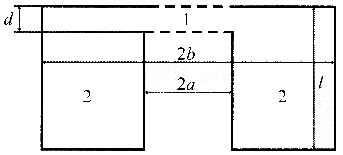
\includegraphics[width=0.5\textwidth]{fig/fig2}
	\caption{Поперечное сечение тороидального резонатора: 1 — емкостной объем резонатора, 2 — индуктивный объем резонатора}
	\label{fig:2}
\end{figure}

При наличии потерь энергии поля в резонаторе, возникающих из-за конечной проводимости стенок и отвода мощности в нагрузку, свободные колебания резонатора являются затухающими, при этом в рамках метода комплексных амплитуд удобно вводить комплексную частоту $\omega = w^{\prime}+i\omega ^{\prime \prime}$. Ве­
личина $\omega ^{ \prime \prime }$ может быть выражена через добротность резонатора, которая, как правило, измеряется экспериментально.

В клистронах применяются резонаторы, допускающие механическую перестройку резонансной частоты. Наиболее распространены два способа перестройки: индуктивный и емкостной. Индуктивная перестройка осуществляется введением в область магнитного поля металлических поршней, кото­рые, уменьшая занятый полем объем, уменьшают индуктивность резонатора и тем самым повышают его резонансную частоту. Емкостная перестройка может быть осуществлена путем деформации гибкой мембраны. Сближение сеток резонатора, обеспечиваемое прогибом мембраны, ведет к увеличению емкости зазора и уменьшению резонансной частоты. Механические способы перестройки обеспечивают отстройку от основной частоты на 20-25\%.

\subsection{Модуляция скорости электронов в пучке}

Рассмотрим процесс модуляции электронного потока по скорости. В установившемся режиме колебания в резонаторе близки к гармоническим, поле в зазоре имеет вид 
$E = E _ { z } = E _ { m } \text { sin } \omega t$, 
где $E _ { m } = \frac { U _ { m } } { d }$, $U _ { m }$ амплитуда напряжения на зазоре,$E _ { z }$ проекция электрического ноля на ось $z$,
$d$ - ширина зазора, $\omega$ частота стационарных колебаний. Найдем приращение энергии электрона, прошедшего через зазор. Кинетическая энергия,
приобретаемая одиночным электроном при прохождении пути $\dd z$ внутри за­зора, равна работе силы электрического поля: 
$\dd W = - e \frac { U _ { m } } { d } \sin \omega t \dd z$, 
где $e$ - модуль заряда электрона (знак заряда учтен в явном виде)
\footnote{Если напряжение (потенциал второй сетки относительно первой) $U = -U_m \sin \omega t$ положительно, оно ускоряет электрон, движущийся в положительном направлении оси z.}. 
Электрон, прошедший расстояние между катодом и резонатором, имеет кинетическую энергию 
$\frac { m v _ { 0 } ^ { 2 } } { 2 } = e U _ { 0 }$ , где $U_0 > 0$-- потенциал резонатора относительно ка­тода, $v_0$ — скорость электрона, $m$ — его масса. Отсюда при условии $v _ { 0 } \ll c$ имеем
\footnote{Пренебрежение релятивистскими поправками возможно до значений $U_0$ порядка нескольких
десятков киловольт.} 
$v _ { 0 } = \sqrt { \frac { 2 e U _ { 0 } } { m } }$

При выполнении условия 
$\frac { U _ { m } } { U _ { 0 } } \ll 1$ возмущения скорости $v_0$ под воздействием высокочастотного поля незначительны. Поэтому если $t_0$ — время про­
хождения электроном центра зазора, то время его нахождения в точке с координатой $z$ есть $t = t _ { 0 } + \frac { z } { v _ { 0 } }$. Полное приращение энергии имеет вид

\begin{equation}
	 { \Delta W = \int\limits _ { - d / 2 }^{{ + d / 2 }} \frac { - e U _ { m } } { d } \sin \left( \omega t _ { 0 } + \frac { \omega z } { v _ { 0 } } \right) d z = } \\ 
	 { - e U _ { m } \sin \omega t _ { 0 } \frac { \sin \left( \theta _ { 3 } / 2 \right) } { \theta_ { 3 } / 2 } = - e M U _ { m } \sin \omega t _ { 0 }, } 
\end{equation}

где $\theta _ { 3 } = \frac { \omega d } { t _ { 0 } }$ - невозмущенный угол пролета электрона через модулирующий зазор, $M = \frac { \sin \left( \theta _ { 3 } / 2 \right) } { \theta _ { 3 } / 2 }$ - коэффициент взаимодействия электронного потока с полем зазора. Полная кинетическая энергия электрона, вошедшего в зазор с начальной скоростью на выходе из него может быть представлена в виде:
\begin{equation}
	W = \frac { m v ^ { 2 } } { 2 } = \frac { m v_0 ^ { 2 } } { 2 } + \Delta W = e U _ { 0 } + \Delta W.
\end{equation}
Таким образом, скорость электрона на выходе из зазора оказывается равной
\begin{equation}
	v = \sqrt { \frac { 2 e } { m } U _ { 0 } } \left( 1 - \frac { M U _ { m } } { U _ { 0 } } \sin \omega t _ { 0 } \right) ^ { 1 / 2 }.
\end{equation}
При выполнении условия $\frac { U _ { m } } { U _ { 0 } } \ll 1$ можно разложить выражение для $v$ в ряд Тейлора и ограничиться двумя первыми членами ряда:
\begin{equation}
	v = \sqrt { \frac { 2 e } { m } U _ { 0 } } \left( 1 - \frac { 1 } { 2 } \frac { M U _ { m } } { U _ { 0 } } \sin \omega t _ { 0 } + \ldots \right) \approx v _ { 0 } - v _ { 1 } \sin \omega t _ { 0 },
\end{equation} где $v _ { 1 } = \frac { M U _ { m } } { 2 U _ { 0 } } v _ { 0 }$
Из полученного выражения видно, что скорость электро­на на выходе из зазора определяется фазой поля, существовавшей в момент прохождения им центра зазора. Наибольшая амплитуда скоростной модуляции $v_1$ достигается при стремлении коэффициента взаимодействия $M$ к единице, что выполняется при стремлении $\theta_3$ к нулю.

\subsection{Модуляция электронного пучка по плотности}

В пространстве между резонатором и отражателем электроны двигаются в статическом тормозящем поле. Уравнение движения имеет вид 
$mz''- e \frac { U _ { 0 } - U _ { \text{отр} } } { L }$ где $U_{\text{отр}} < 0$ — напряжение на отражателе, $L$ — расстояние между резонатором и отражателем. Интегрируя первый раз уравнение движения и учитывая выражение для скорости $v$ при выходе из зазора, имеем
\begin{equation}
	z ^ { \prime } = v - \frac { e } { m } \frac { U _ { 0 } - U _ { \text { отр } } } { L } \left( t - t ^ { \prime } \right)
\end{equation}
где $t'$ — момент выхода электрона из зазора. Через t в дальнейшем будем обозначать момент, когда тот же электрон возвращается в плоскость второй сетки. Повторное интегрирование уравнения (5) дает
\begin{equation}
	z = v \left( t - t ^ { \prime } \right) - \frac { e } { m } \frac { U _ { 0 } - U _ { \text { отр } } } { L } \frac { \left( t - t ^ { \prime } \right) ^ { 2 } } { 2 } + \frac { d } { 2 }
\end{equation}

Время пролета электрона в пространстве группировки можно найти из условия $z = d / 2$ при $t=t''$, откуда следует, что 
$t ^ { \prime \prime } - t ^ { \prime } = 0$ и 
$\frac { e } { m } \frac { U _ { 0 } - U _ { \text { отр } } } { L }\cdot \frac { \left( t ^ { \prime \prime } - t ^ { \prime } \right) } { 2 v } = 1$
Первое решение $(t' = t'' )$ соответствует моменту вылета электрона из зазора, второе дает время его пролета в тормозящем поле:
\begin{equation}
	t ^ { \prime \prime } - t ^ { \prime } = \frac { 2 m } { e } \frac { v L } { L _ { 0 } - U _ { \text { отр } } }
\end{equation}

При выполнении условия $U_{ m } / U _{ 0 } \ll 1$ время пролета в зазоре определяется скоростью $v_0$, поэтому связь времени вылета электрона из зазора со временем его нахождения в центре зазора можно приближенно записать в виде
$t'' = t _ { 0 } + d / \left( 2 v _ { 0 } \right)$. Таким образом, подставляя выражение для скорости (4) в (7), получим
\begin{equation}
	t ^ { \prime \prime } = t ^ { \prime } + \frac { 2 m L } { e \left( U _ { 0 } - U _ { \text { отр } } \right) } \left( v _ { 0 } - \frac { M U _ { m } } { 2 U _ { 0 } } v _ { 0 } \sin \left( \omega t ^ { \prime } - \frac { \omega d } { 2 v _ { 0 } } \right) \right)
\end{equation}

Из найденного выражения видно, что время пролета электронов в пространстве группировки зависит от фазы высокочастотного напряжения, существующего в момент пролета электроном середины зазора, и от амплитуды этого напряжения.

На рис.\ref{fig:3} представлены примеры пространственно-временных диаграмм(зависимостей координат электронов от времени) для таких значений потенциалов на резонаторе и отражателе, при которых электроны, вышедшие из резонатора в различные моменты времени, возвращаются в него одновремен­но, образуя сгусток. Сверхвысокочастотное поле в резонаторе в рассматриваемых в случаях в момент времени пролета сгустка максимально и является для него тормозящим. Уменьшение кинетической энергии электронов при этом приводит к возрастанию энергии СВЧ поля. Разумеется, при других значениях потенциалов на электродах клистрона сгусток может сформироваться и вне зазора резонатора, при этом эффективная передача энергии от пучка полю становится невозможной.

Домножим соотношение (8) на ы и введем следующие величины:
\begin{equation}
	\theta _ { \text{г} } = \frac { 2 m } { e } \frac { v _ { 0 } \omega L } { U _ { 0 } - U _ { \text{ oтр } } }
\end{equation} — угол пролета электрона в пространстве группировки,
\begin{equation}
	X = \theta _ { \text{г} } \frac{M U _ { m } } { 2 U _ { 0 } }
\end{equation} — параметр группировки. В результате получим выражение, связывающее время возвращения электрона в плоскость второй сетки $(t'' )$ со временем выхода электрона из зазора $(t')$:
\begin{equation}
	\omega t ^ { \prime \prime } = \omega t ^ { \prime } + \theta _ { r } - X \sin \left( \omega t ^ { \prime } - \frac { \theta _ { 3 } } { 2 } \right)
\end{equation}
Соотношение (11) является исходным для нахождения конвекционного тока пучка электронов.

\begin{figure}[h!]
	\centering
	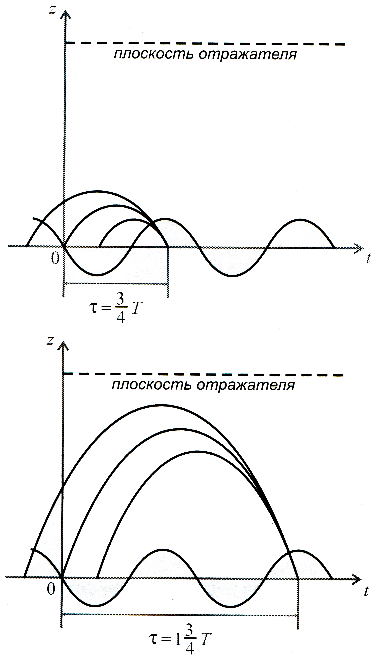
\includegraphics[width=0.5\textwidth]{fig/fig3}
	\caption{Пространственно-временные диаграммы движения электронов при двух значениях оптимального времени пролета $\tau$ в пространстве группировки ($z=0$ координата, соответствующая середине зазора)}
	\label{fig:3}
\end{figure}

\subsection{Возбуждение резонатора клистрона током пучка}
Сгруппированный электронный пучок формирует ток $I$, возбуждающий колебания в резонаторе. При этом условие возбуждения клистрона принимает следующий вид:
\begin{equation}
	\pi + 2 \pi n < \left( \theta _ { 3 } + \theta _ { \text{г} } \right) < 2 \pi ( n + 1 )
\end{equation}где $n=1,2,3,\dots $.

Указанные интервалы углов пролета, при которых возможна генерация, носят название зон генерации клистрона. В центре зон генерации, т. е. при
$\theta _ { \text{г} } + \theta _ { \text{з} } = 2 \pi ( n + 3 / 4 )$ амплитуда максимальна, а на краях равна нулю. Угол пролета в пространстве группировки $\theta _ { \text{г} }$ можно варьировать, изменяя ли­бо напряжение на резонаторе, либо напряжение на отражателе (см. (9)).
Пространственно-временные диаграммы, соответствующие двум оптималь­ным углам пролета, представлены на рис.\ref{fig:3}.

Одной из важных характеристик клистрона является пусковой ток — значение тока $I_0$, при котором клистрон возбуждается:

\begin{equation}
	I _ { 0 \, \text { пуск } } = - \frac { 2 U _ { 0 } G } { M ^ { 2 } 
	\theta _ { \text{ г } } \sin \left( \theta _ { \text{з} } + \theta _ { \text{ г } } \right) }
\end{equation} где G — действительная часть проводимости резонатора.

Как видаю из соотношения (13), пусковой ток клистрона тем меньше, чем меньше величина G. С ростом номера зоны самовозбуждение клистрона облегчается. Ток, требующийся для самовозбуждения клистрона, тем меньше, чем ниже ускоряющее напряжение $U_0$. Легче всего клистрон возбуждается в центрах зон. Напротив, на их краях 
$\sin \left( \theta _ { \text{з} } + \theta _ { \text{г} } \right) \rightarrow 0$ и 
$I _ { 0\, \text { пуск } } \rightarrow \infty$.

\section{Экспериментальная часть}

Исследуемый клистрон предназначен для работы в десятисантиметровом диапазоне.

На рис. \ref{fig:4} показана схема включения клистрона. С блока питания (выпрямители I, II, III) напряжение подается на отражатель, резонатор и управляющий электрод. Контроль величин напряжений на электродах клистрона осуществляется по вольтметру, последовательно подключаемому с помощью
переключателя П1 к любому из электродов. К отражателю клистрона с по­мощью переключателя П2 может подключаться генератор пилообразного
напряжения; СВЧ колебания, генерируемые отражательным клистроном, с помощью петли связи через ответвитель подводятся к кристаллическому
детектору и волномеру ВМТ-10. В цепи детектора стоит микроамперметр, показания которого пропорциональны уровню выходной мощности клистрона
\footnote{При наблюдении зон генерации клистрона на экране осциллографа переключатель П2 ставится  в положение <<модуляция>> (<<Вкл>>), П3--в положение <<Выкл>>(<<Осциллограф>>)}.
\begin{figure}[H]
	\centering
	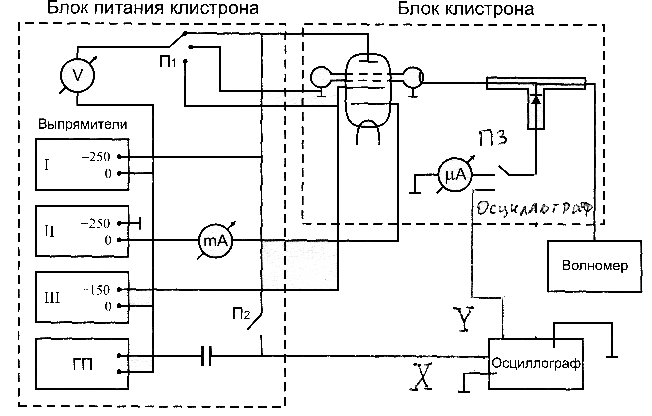
\includegraphics[width=\textwidth]{fig/fig4}
	\caption{ Блок-схема включения клистрона}
	\label{fig:4}
\end{figure}

\subsection{Задания}
\begin{enumerate}
	\item  Включить установку и выставить рабочий режим клистрона, подо­
	брав подходящие значения напряжения на резонаторе (в интервале от 0 до
	-250 В), ускоряющем электроде (от 0 до + 150 В) и отражающем электроде
	(от 0 до —250 В).
	\item  Визуально исследовать режим генерации клистрона на экране осциллографа. Для этого подать на отражатель пилообразное напряжение, поста­
	вив переключатель П2 в положение «модуляция»: На вход Y осциллографа
	подается напряжение с детектора, а на вход X в качестве развертки — пилообразное напряжение с модулятора.
		\begin{enumerate}
			\item Используя кальку, зарисовать зоны генерации клистрона и пронумеровать их. Выяснить, как меняются зоны генерации в зависимости от потенци­
			алов электродов клистрона. Выбрать оптимальный режим работы клистрона (найти значения напряжения на электродах, при которых реализуется
			\item Уменьшая амплитуду пилообразного напряжения на отражателе клистрона, получить на экране только одну зону генерации. Определить с  по­мощью волномера ширину частотной перестройки клистрона. Для этого, из­меняя настройку волномера, проследить на экране осциллографа движение
			метки по зоне генерации. Зафиксировав показания волномера в крайних	точках зоны, определить ширину частотной перестройки клистрона вдоль
			зоны генерации.
		\end{enumerate}
	
	При выполнении остальных заданий переключатель П2 должен быть в	положении «выкл», при этом должен быть выключен и осциллограф.

	\item Снять зависимости тока в цепи детектора (ток пропорционален мощ­
	ности колебаний) от: 
		\begin{enumerate}
			\item напряжения на отражателе (при нескольких фиксированных напряжениях на резонаторе),
			\item напряжения на резонаторе (при нескольких фиксированных напряжениях на отражателе).
		\end{enumerate} 
	Экспериментальные данные представить в виде графиков.
	
	Рекомендуется снятие характеристик в этом задании совмещать с измерением частотных зависимостей (см. задание 4).

	\item Измерить при помощи волномера длину волны колебаний, генерируемых клистроном, и проследить, как она меняется вдоль каждой зоны. Для
	этого снять зависимости частоты от:
		\begin{enumerate}
			\item  напряжения на отражателе (при фиксированном напряжении на резонаторе) ,
			\item  напряжения на резонаторе (при фиксированном напряжении на отражателе).
		\end{enumerate}
	
	Экспериментальные данные представить в виде графиков.

	\item  Снять зависимость тока в цепи детектора от тока пучка для различных зон генерации клистрона. Потенциал отражателя для каждой зоны устанавливается по максимальной интенсивности колебаний (т.е. в центре зоны). Экспериментальные данные представить в виде графиков. На основании измерений определить пусковой ток клистрона для каждой зоны. Регулировку	тока пучка осуществлять изменением величины потенциала на управляющем электроде.

	\item  Объяснить полученные экспериментальные данные.

\end{enumerate}
\newpage
\subsection{Задание 2}
Значения напряжения на электродах, при которых наблюдаются три зоны генерации клистрона:
\begin{itemize}
	\item $U_{\text{рез}}=96$ В
	\item $U_{\text{уск}}=126$ В
	\item $U_{\text{отр}}=42$ В
\end{itemize}
\begin{figure}[h!]
	\centering
	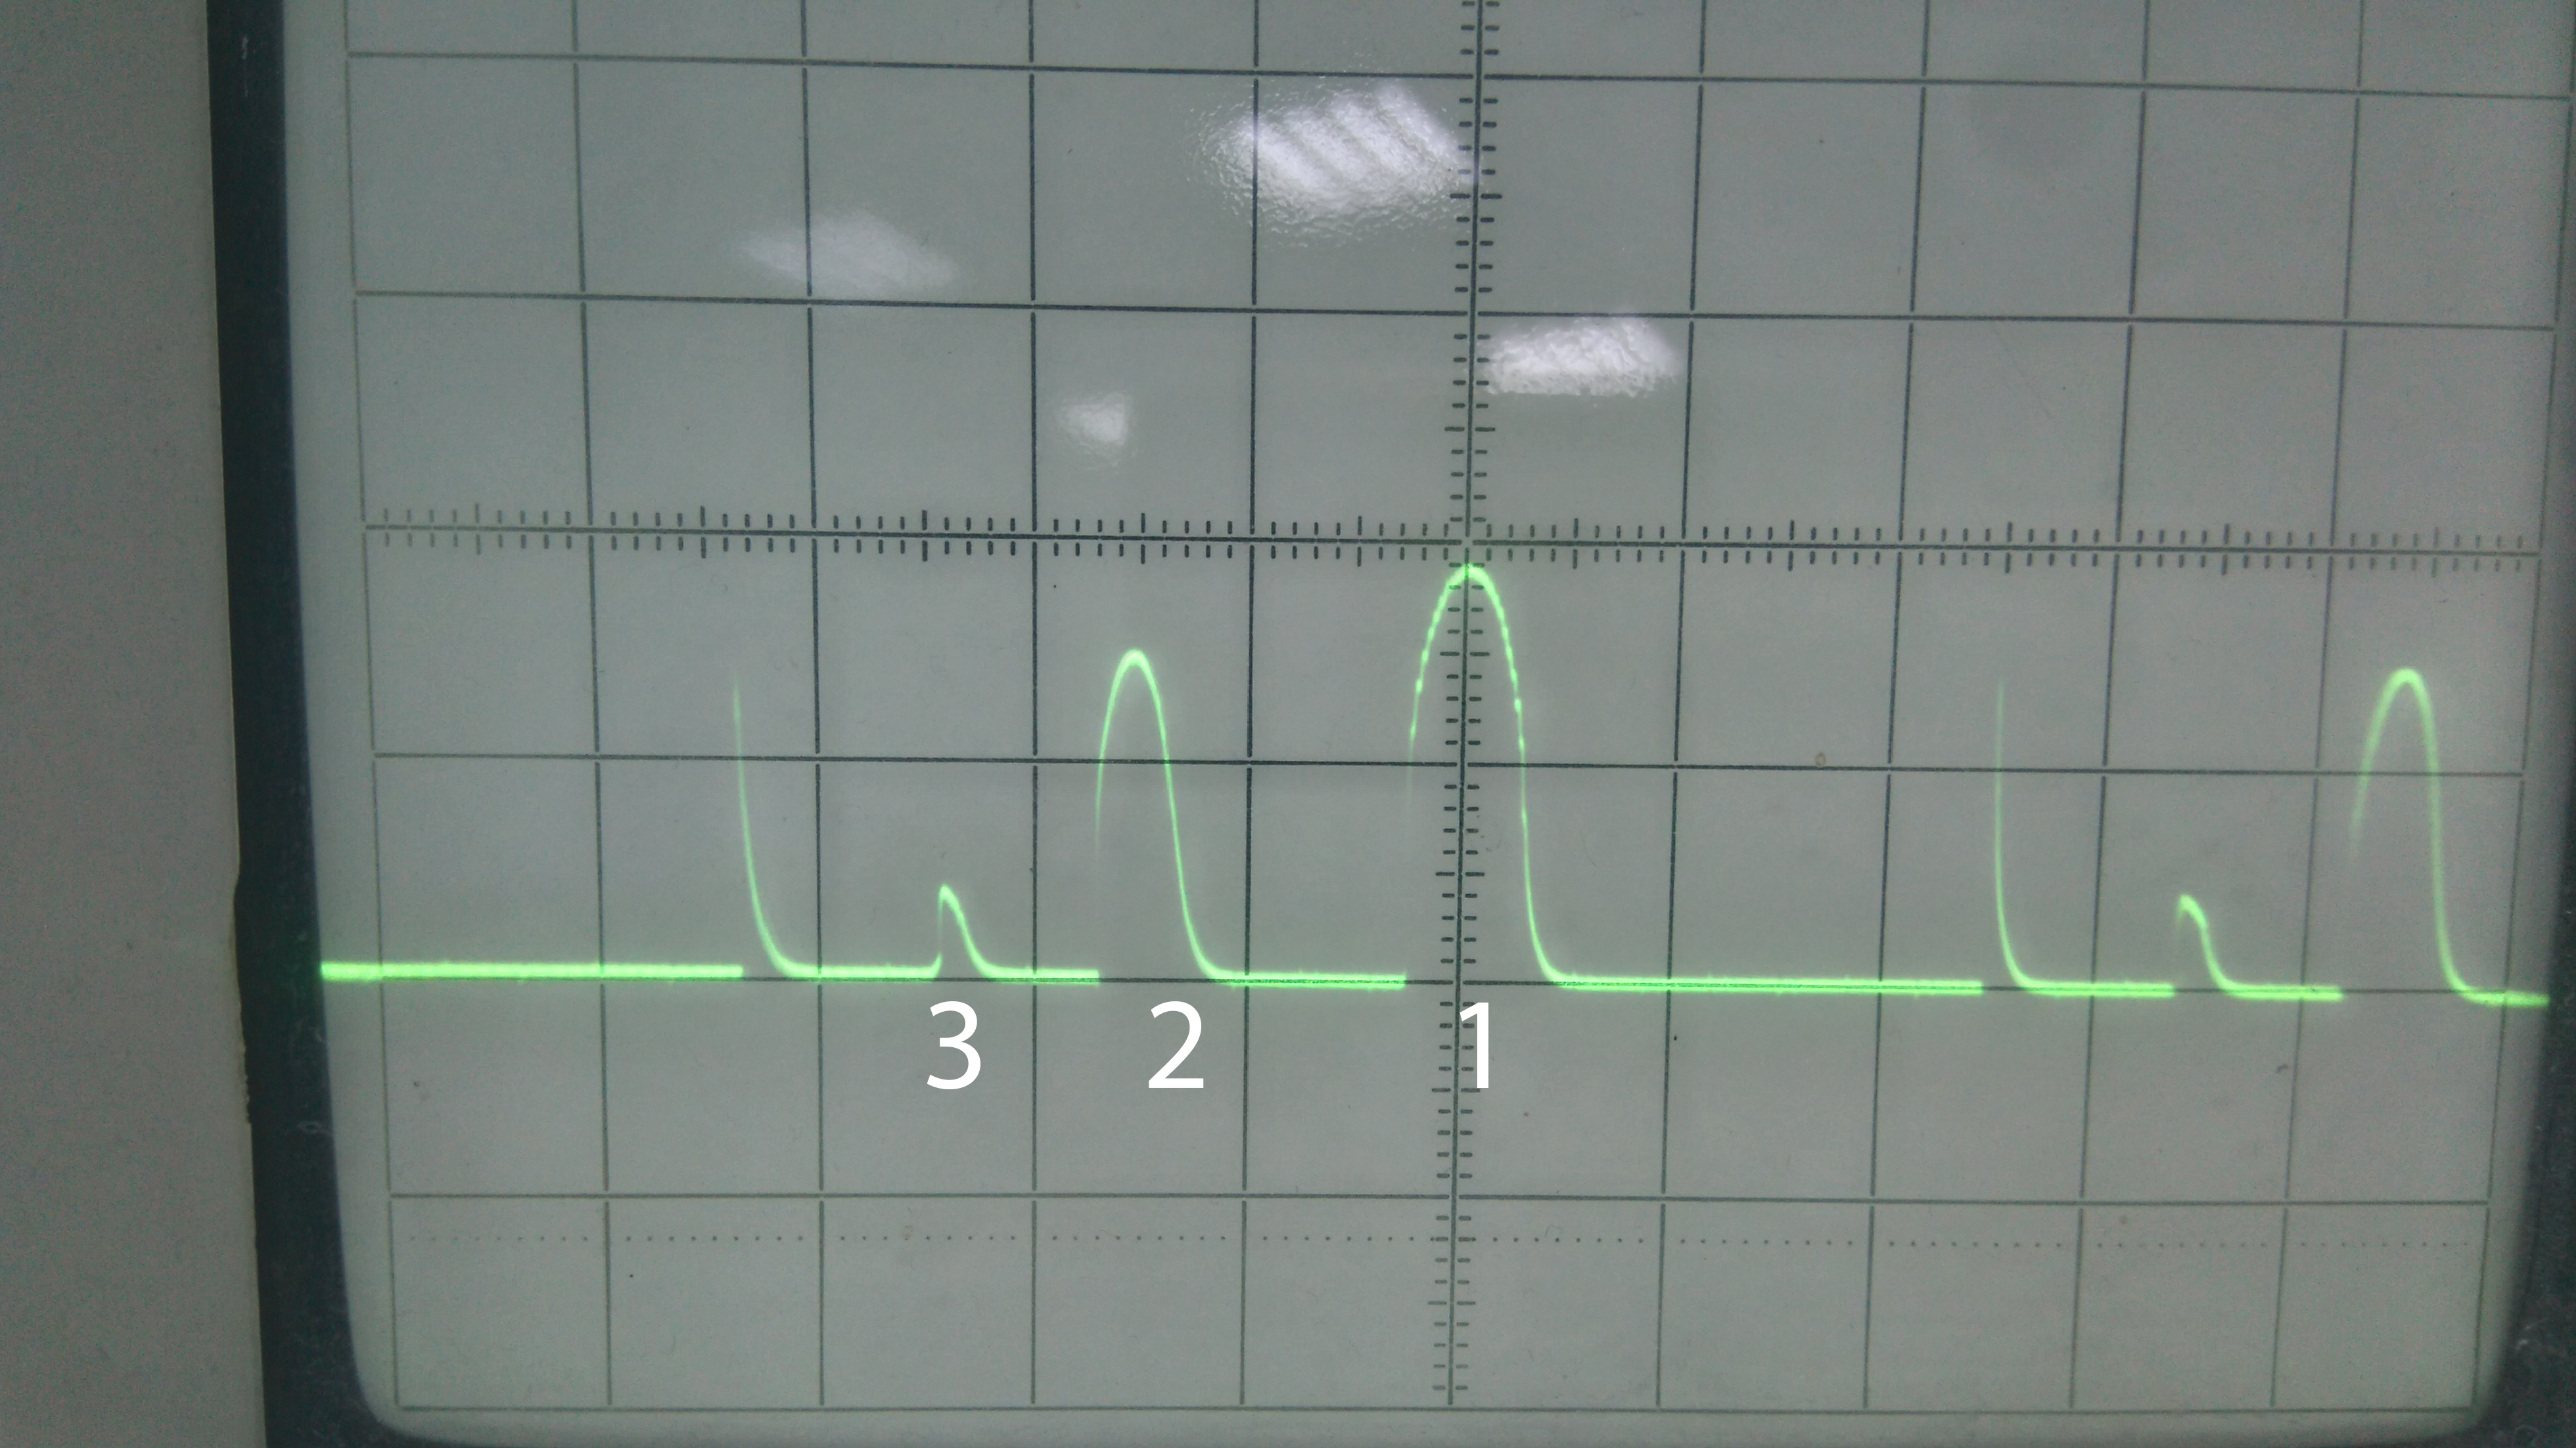
\includegraphics[width=\linewidth]{img/img1}
	\caption{Характерный вид зон генерации клистрона на осциллографе}
	\label{fig:img1}
\end{figure}
\newpage
\begin{figure}[h]
	\begin{minipage}[h]{0.45\linewidth}
		\centering
		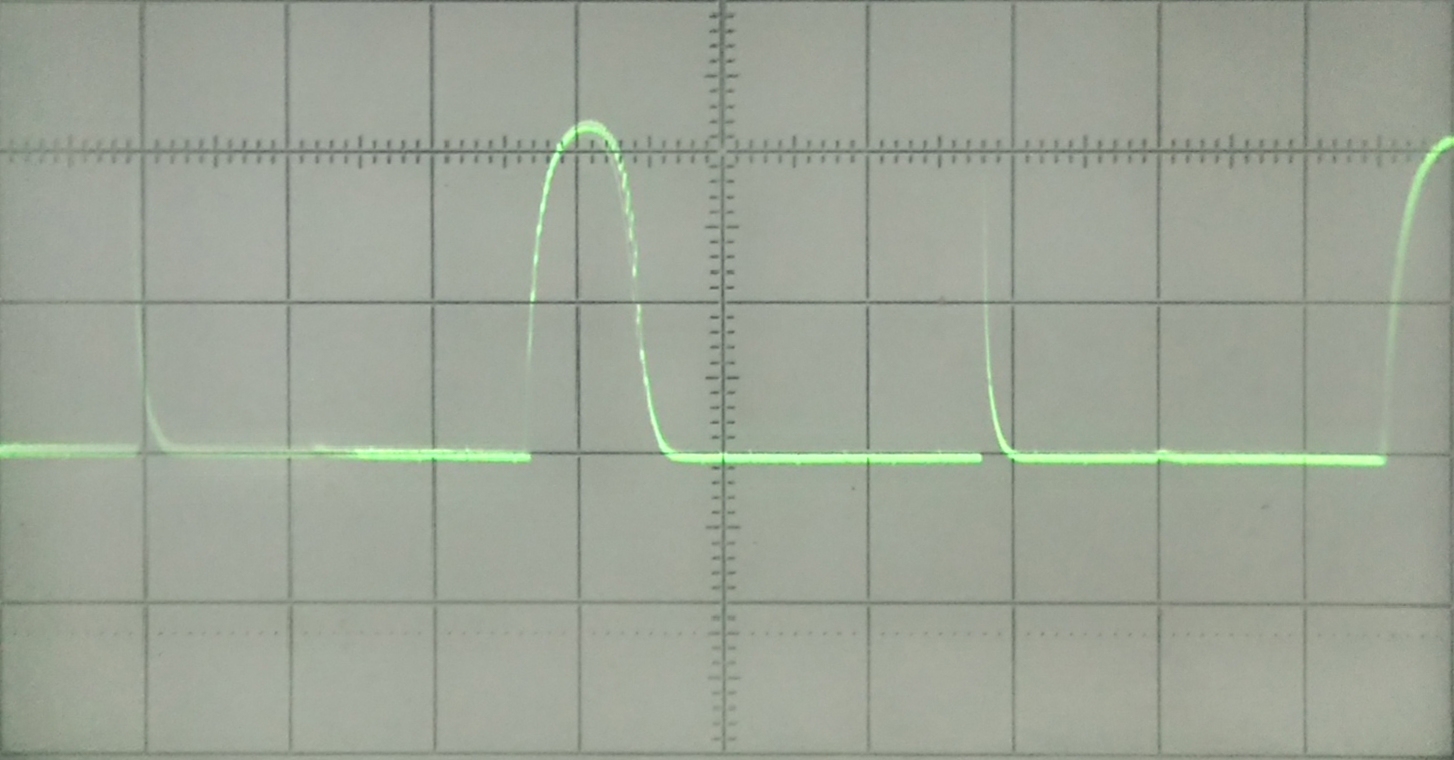
\includegraphics[width=\textwidth]{img/img2}
		\caption{$U_{\text{уск}}=159$ В}
		\label{fig:img2}
	\end{minipage}
	\hfill
	\begin{minipage}[h]{0.45\linewidth}
		\centering
		{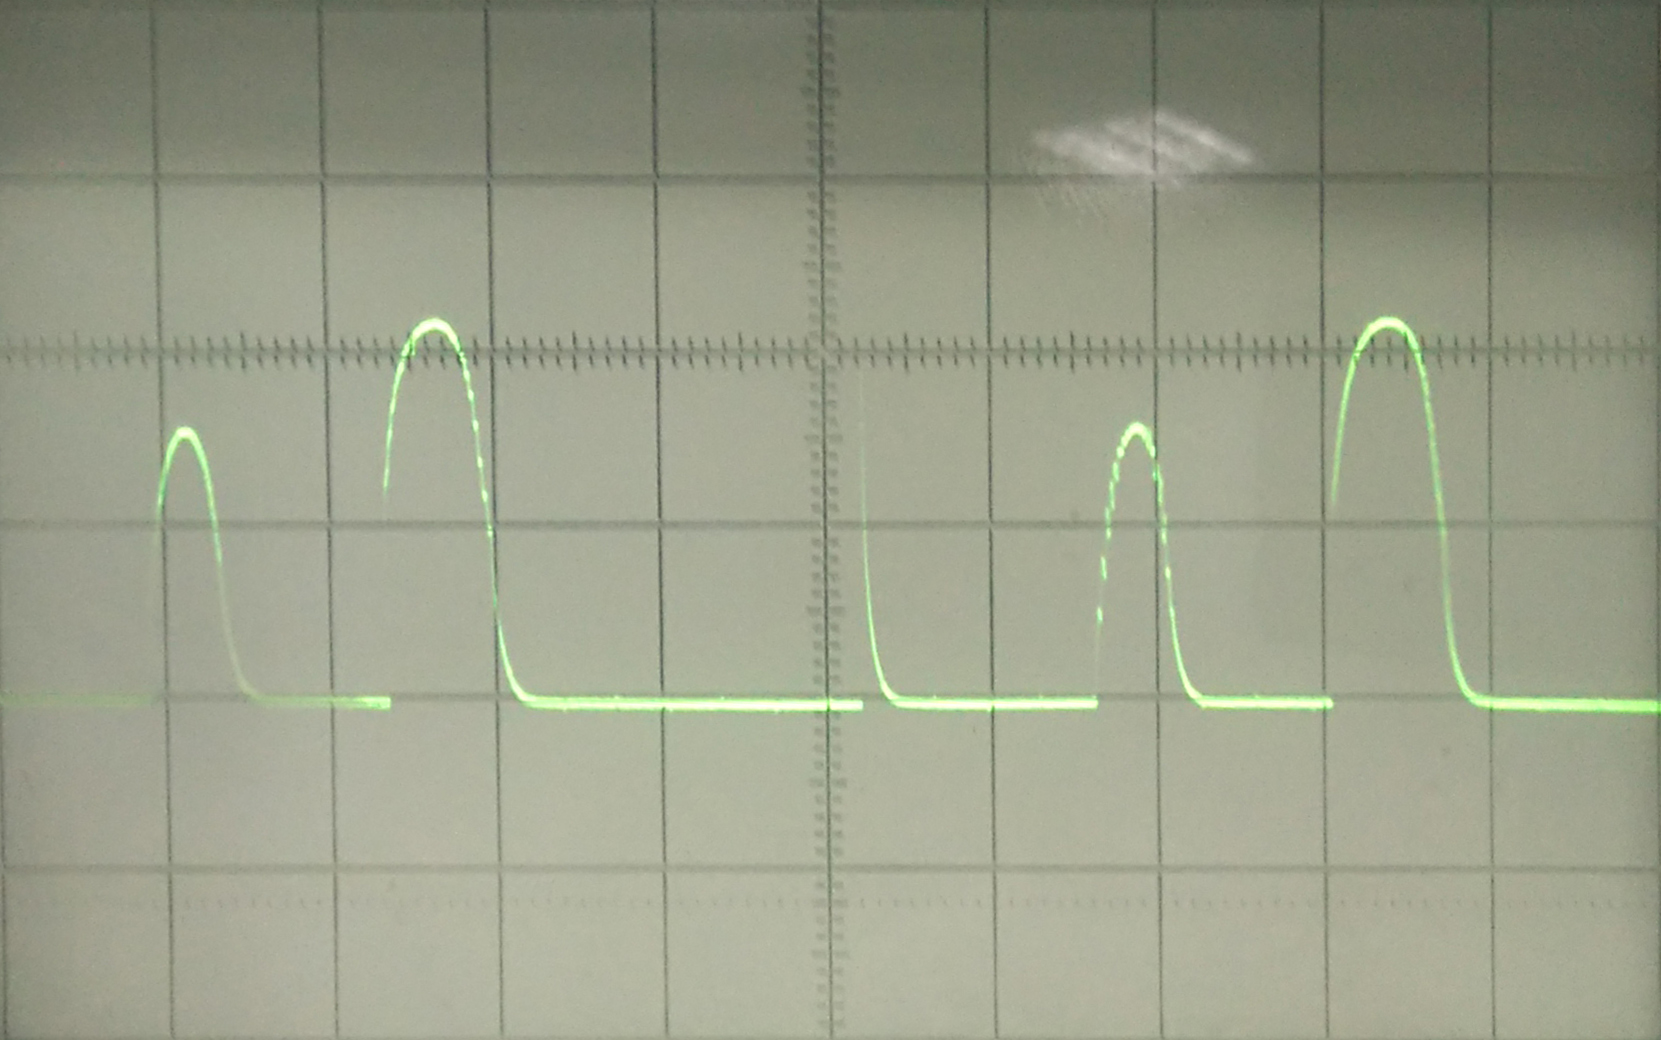
\includegraphics[width=\textwidth]{img/img3}}
		\caption{$U_{\text{уск}}=152$ В}
		\label{fig:img3}
	\end{minipage}
	\vfill
	\vspace{1em}
	\begin{minipage}[h]{0.45\linewidth}
		\centering
		{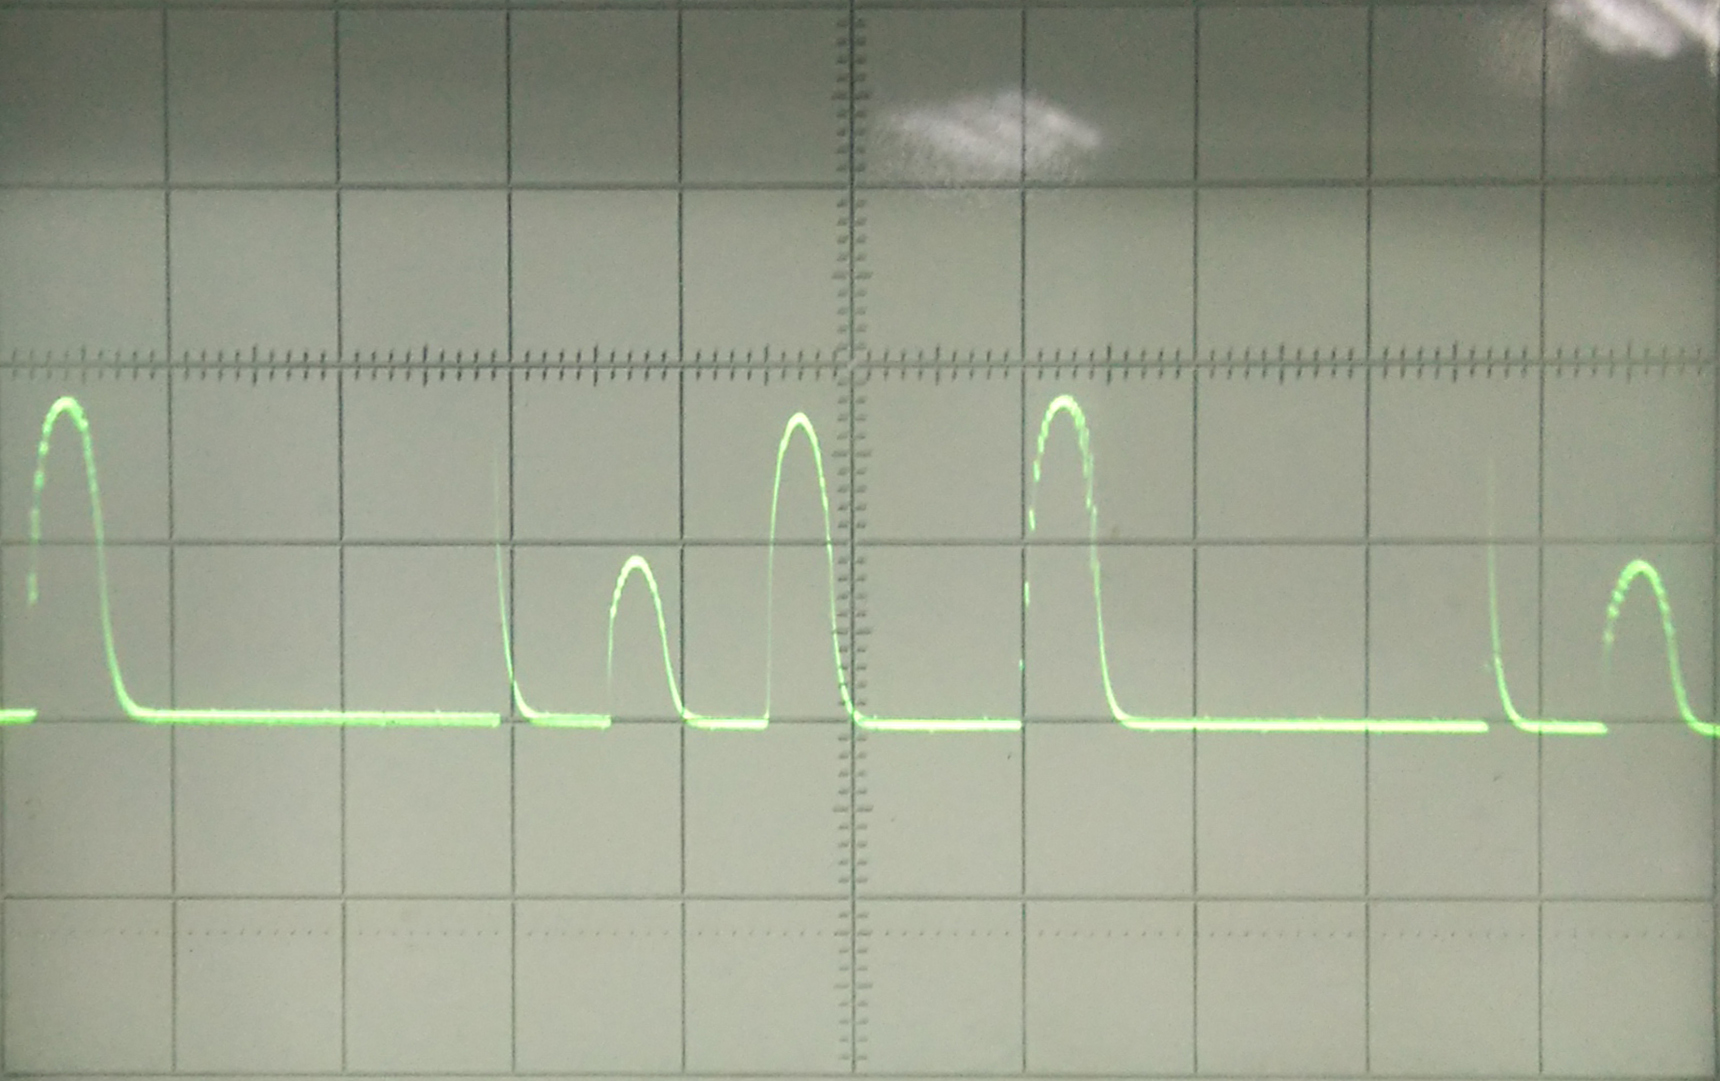
\includegraphics[width=\textwidth]{img/img4}}
		\caption{$U_{\text{уск}}=132$ В}
		\label{fig:img4}
	\end{minipage}
	\hfill
	\begin{minipage}[h]{0.45\textwidth}
		\centering
		{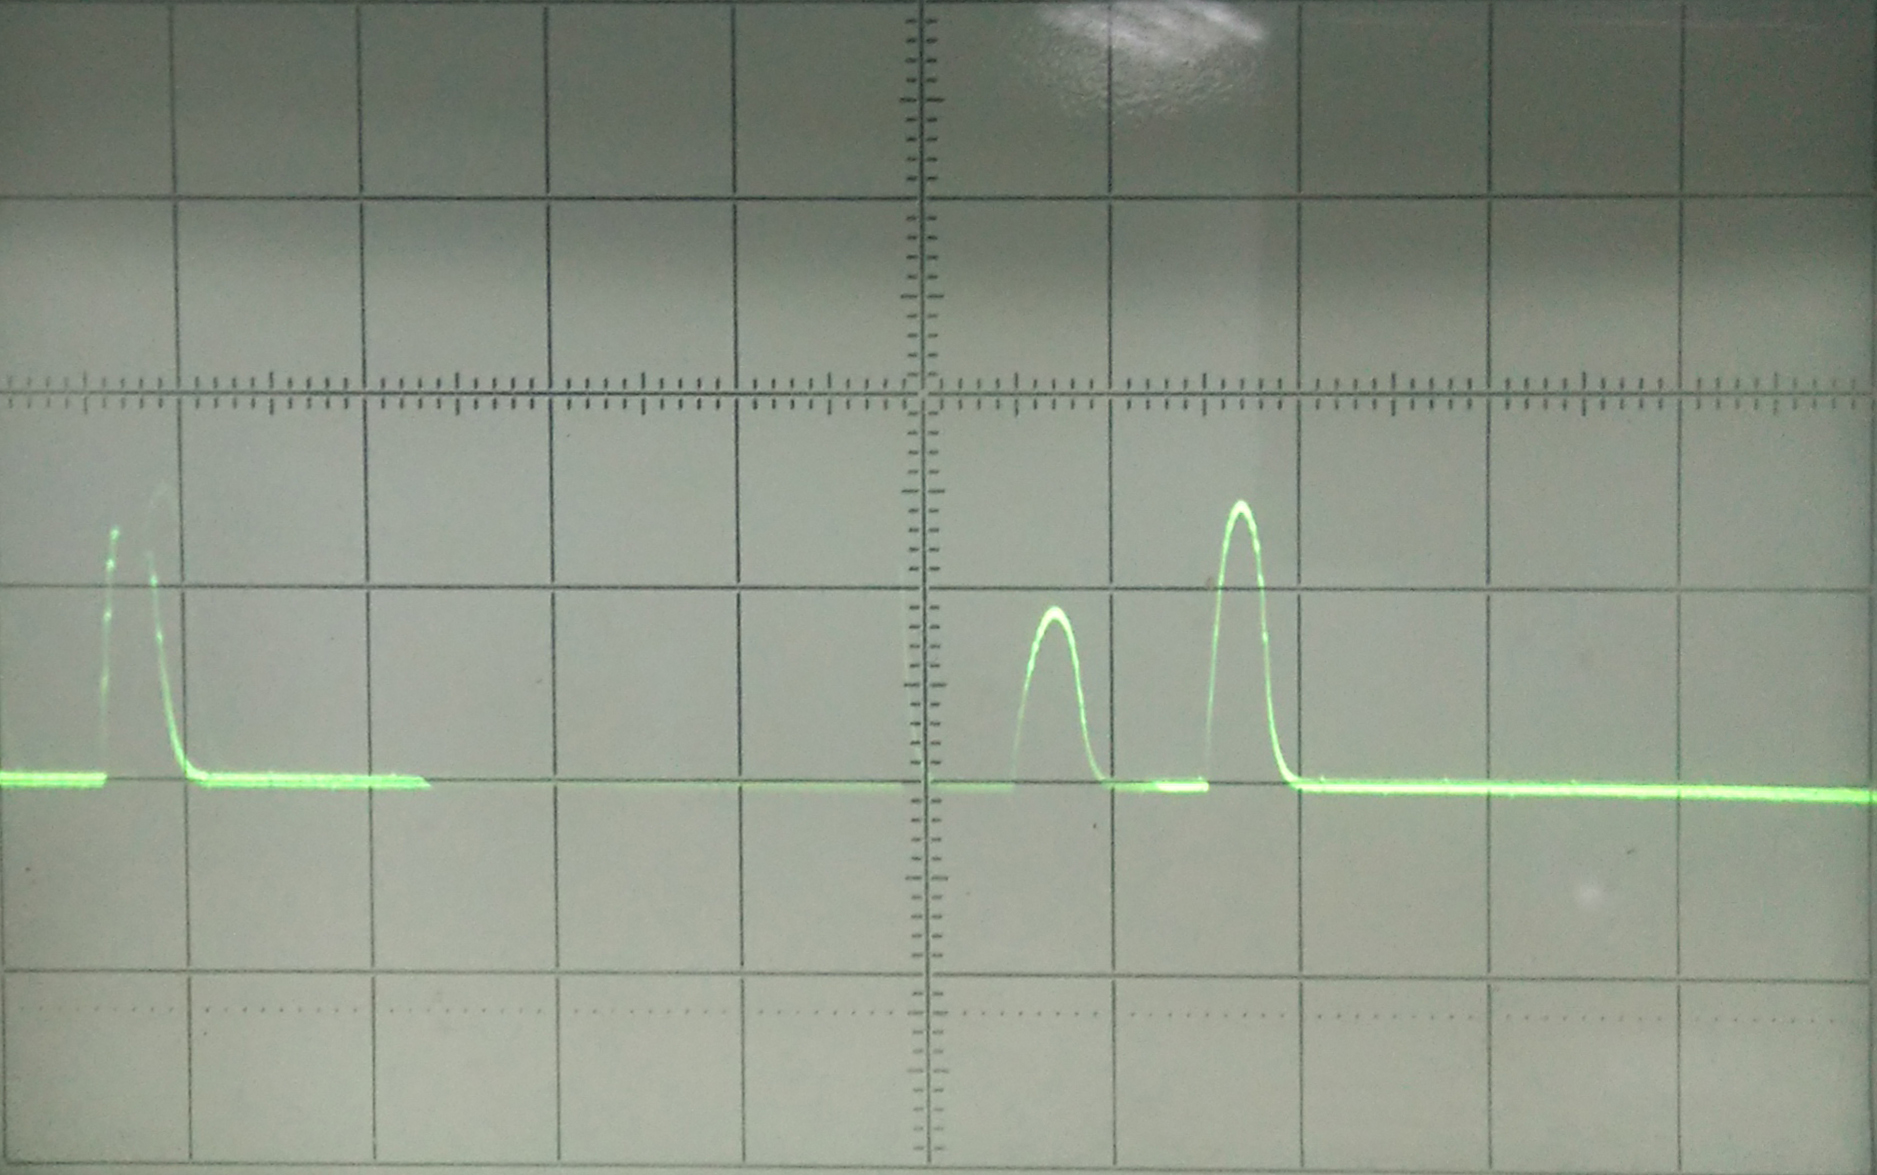
\includegraphics[width=\textwidth]{img/img5}}
		\caption{$U_{\text{уск}}=90$ В}
		\label{fig:img5}
	\end{minipage}

		\begin{minipage}[h]{0.45\textwidth}
		\centering
		{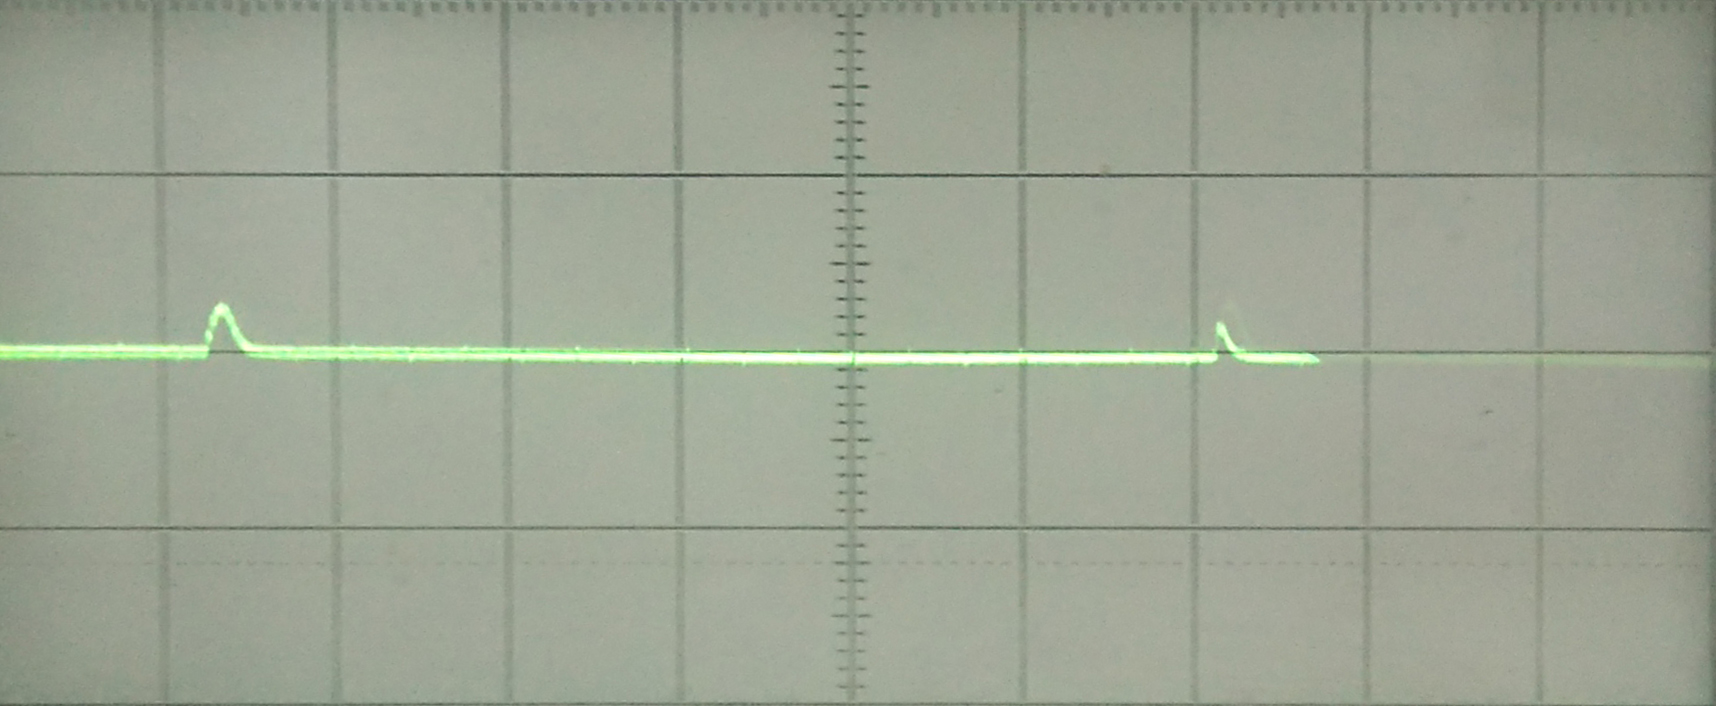
\includegraphics[width=\textwidth]{img/img6}}
		\caption{$U_{\text{уск}}=69$ В}
		\label{fig:img6}
	\end{minipage}
\end{figure}
\newpage


\begin{figure}[h]
	\begin{minipage}[h]{0.45\linewidth}
		\centering
		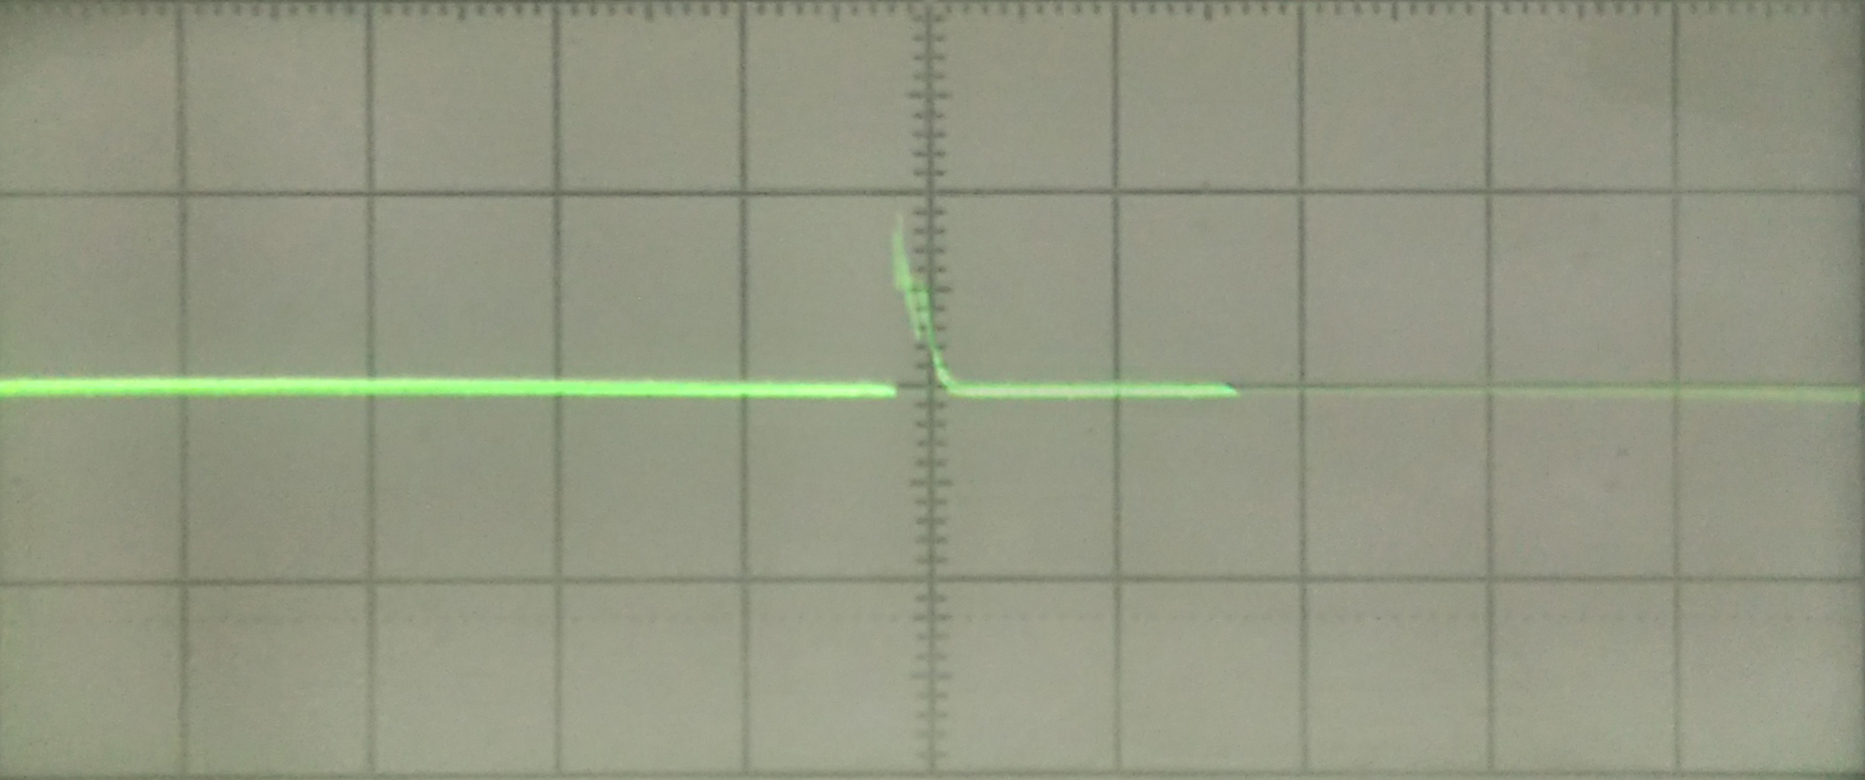
\includegraphics[width=\textwidth]{img/img7}
		\caption{$U_{\text{отр}}=108$ В}
		\label{fig:img7}
	\end{minipage}
	\hfill
	\begin{minipage}[h]{0.45\linewidth}
		\centering
		{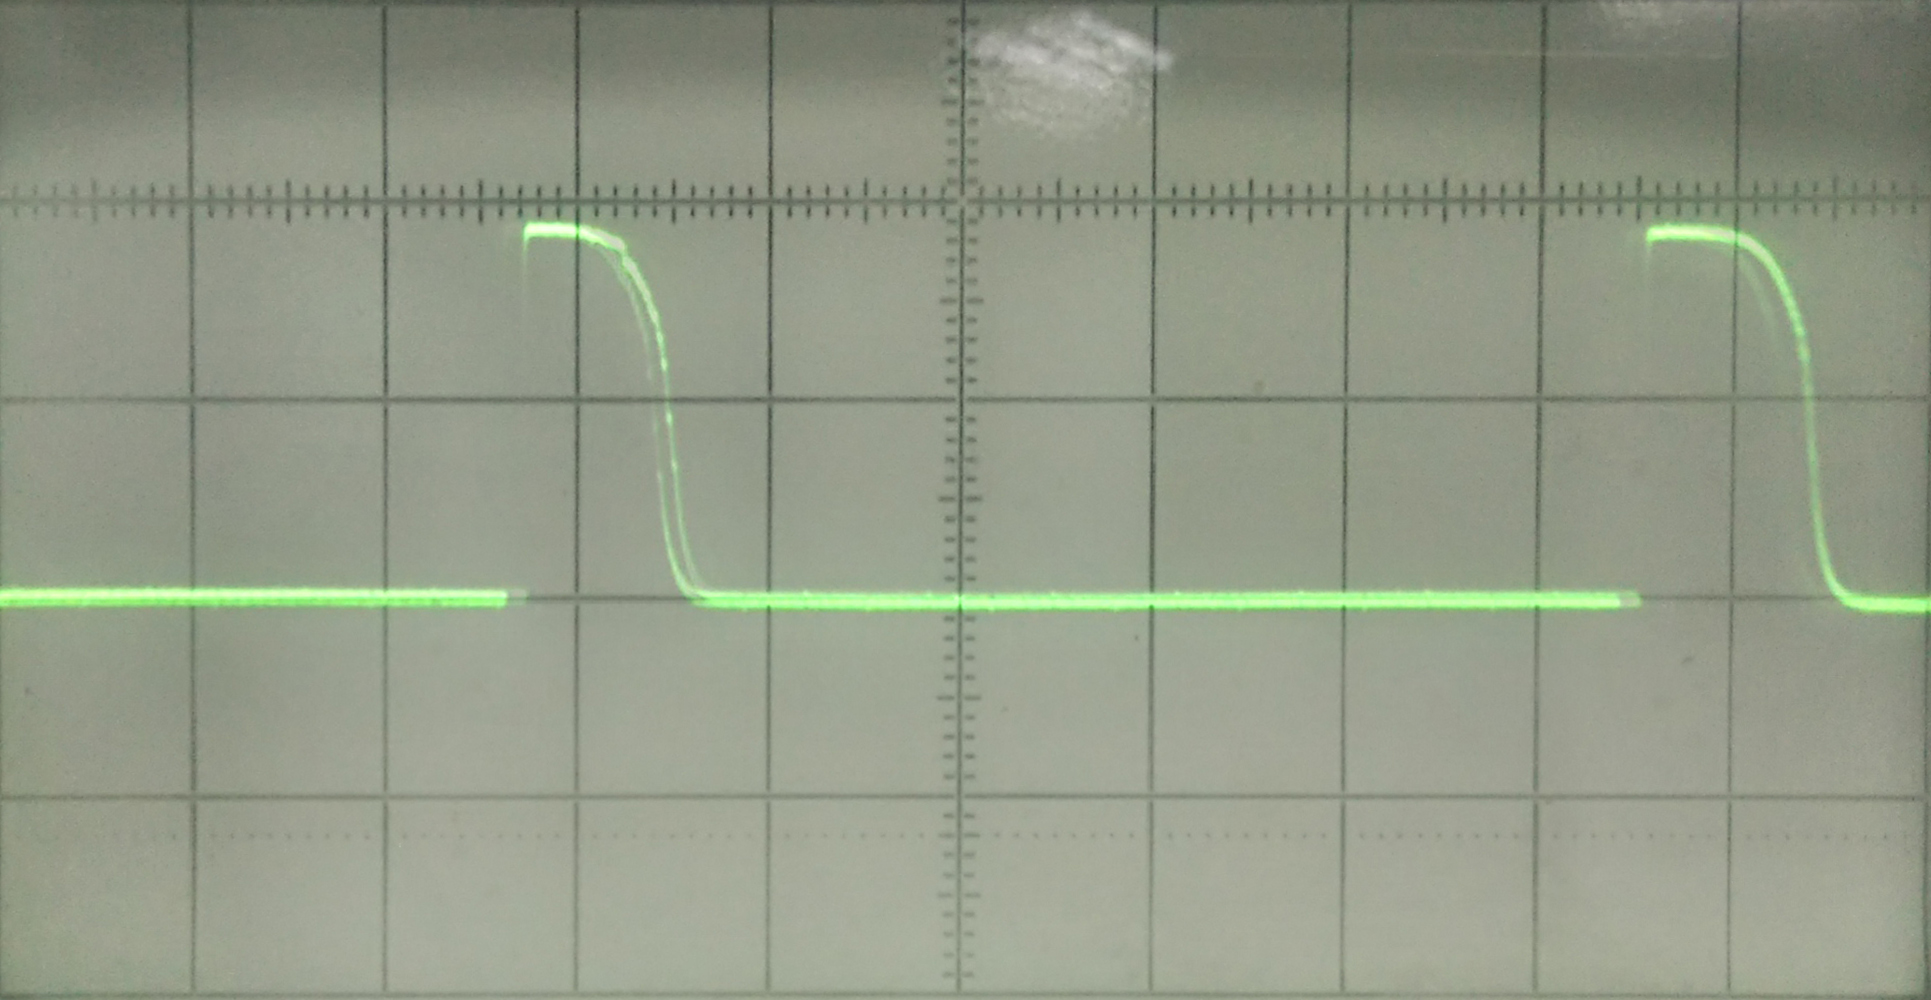
\includegraphics[width=\textwidth]{img/img8}}
		\caption{$U_{\text{отр}}=102$ В}
		\label{fig:img8}
	\end{minipage}
	\vfill
	\vspace{1em}
	\begin{minipage}[h]{0.45\linewidth}
		\centering
		{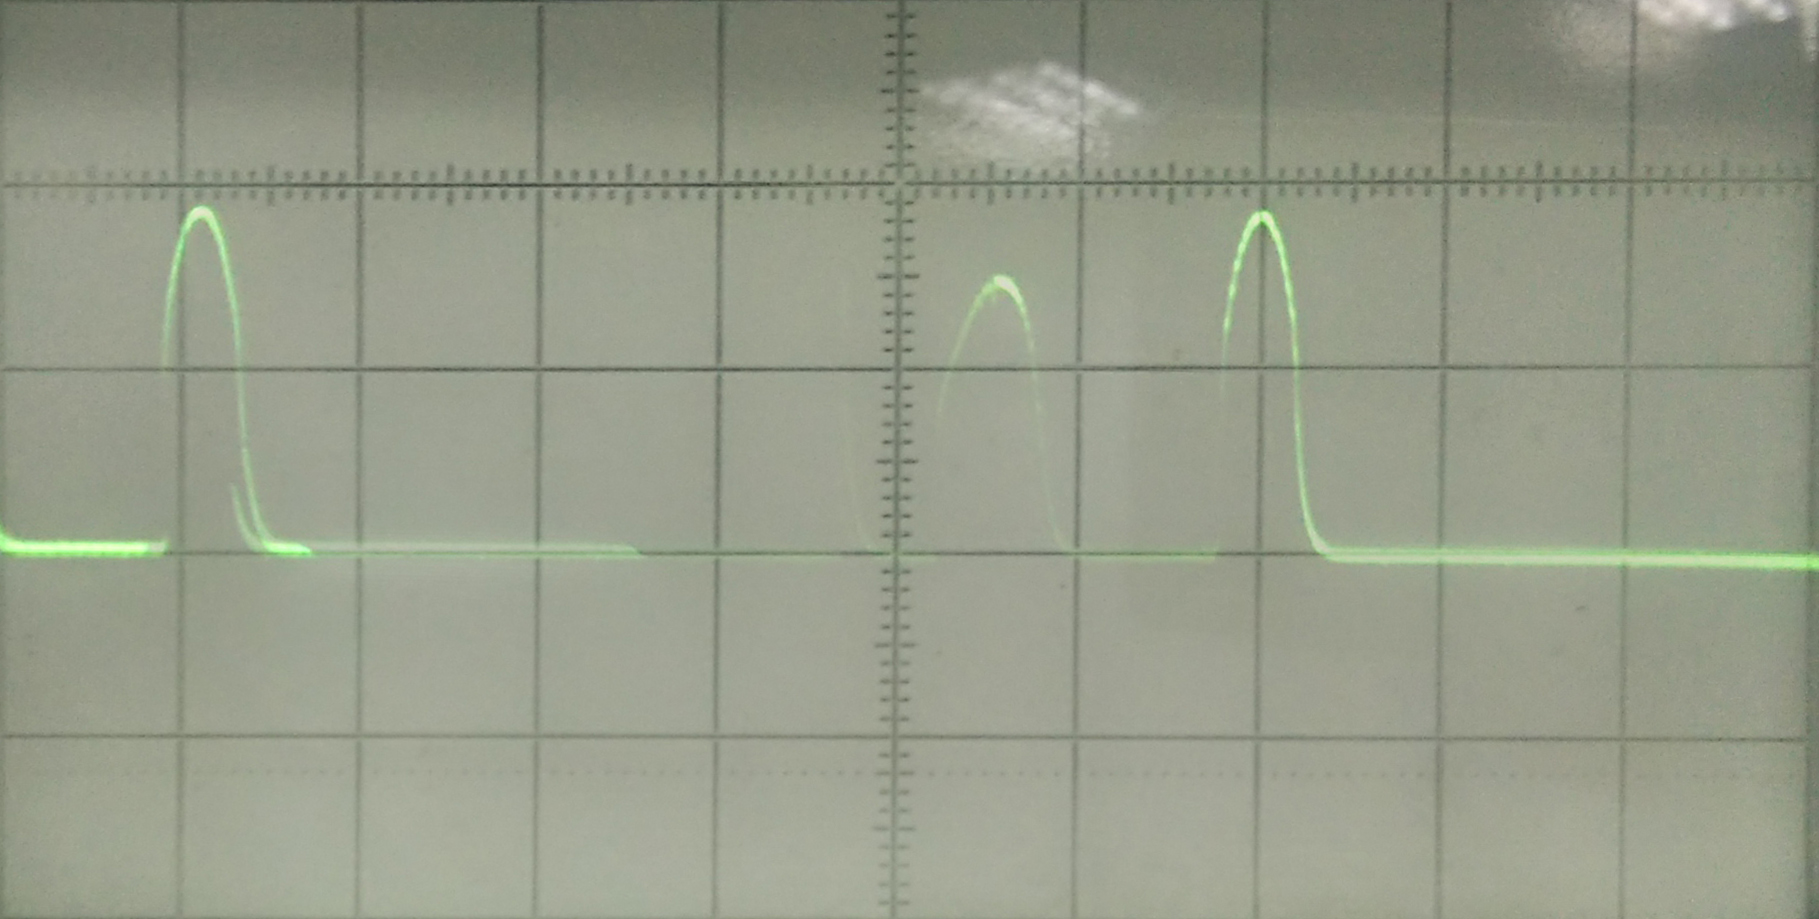
\includegraphics[width=\textwidth]{img/img9}}
		\caption{$U_{\text{отр}}=60$ В}
		\label{fig:img9}
	\end{minipage}
	\hfill
	\begin{minipage}[h]{0.45\textwidth}
		\centering
		{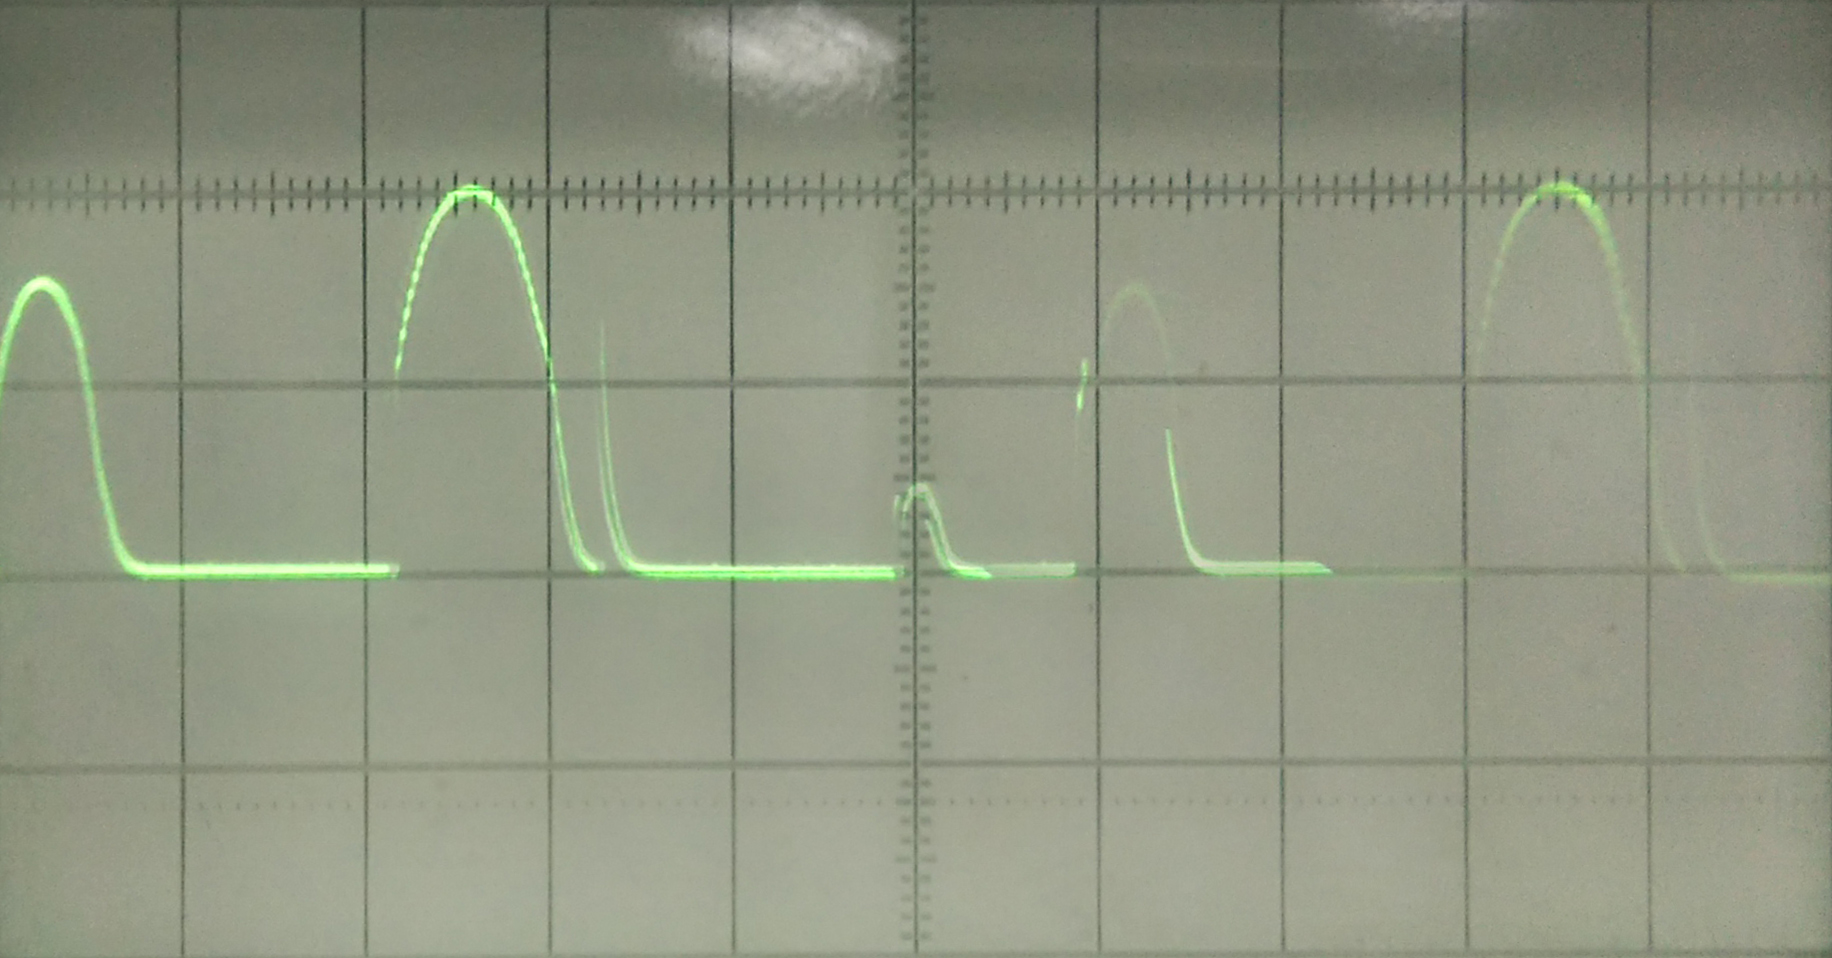
\includegraphics[width=\textwidth]{img/img10}}
		\caption{$U_{\text{отр}}=24$ В}
		\label{fig:img10}
	\end{minipage}

		\begin{minipage}[h]{0.45\textwidth}
		\centering
		{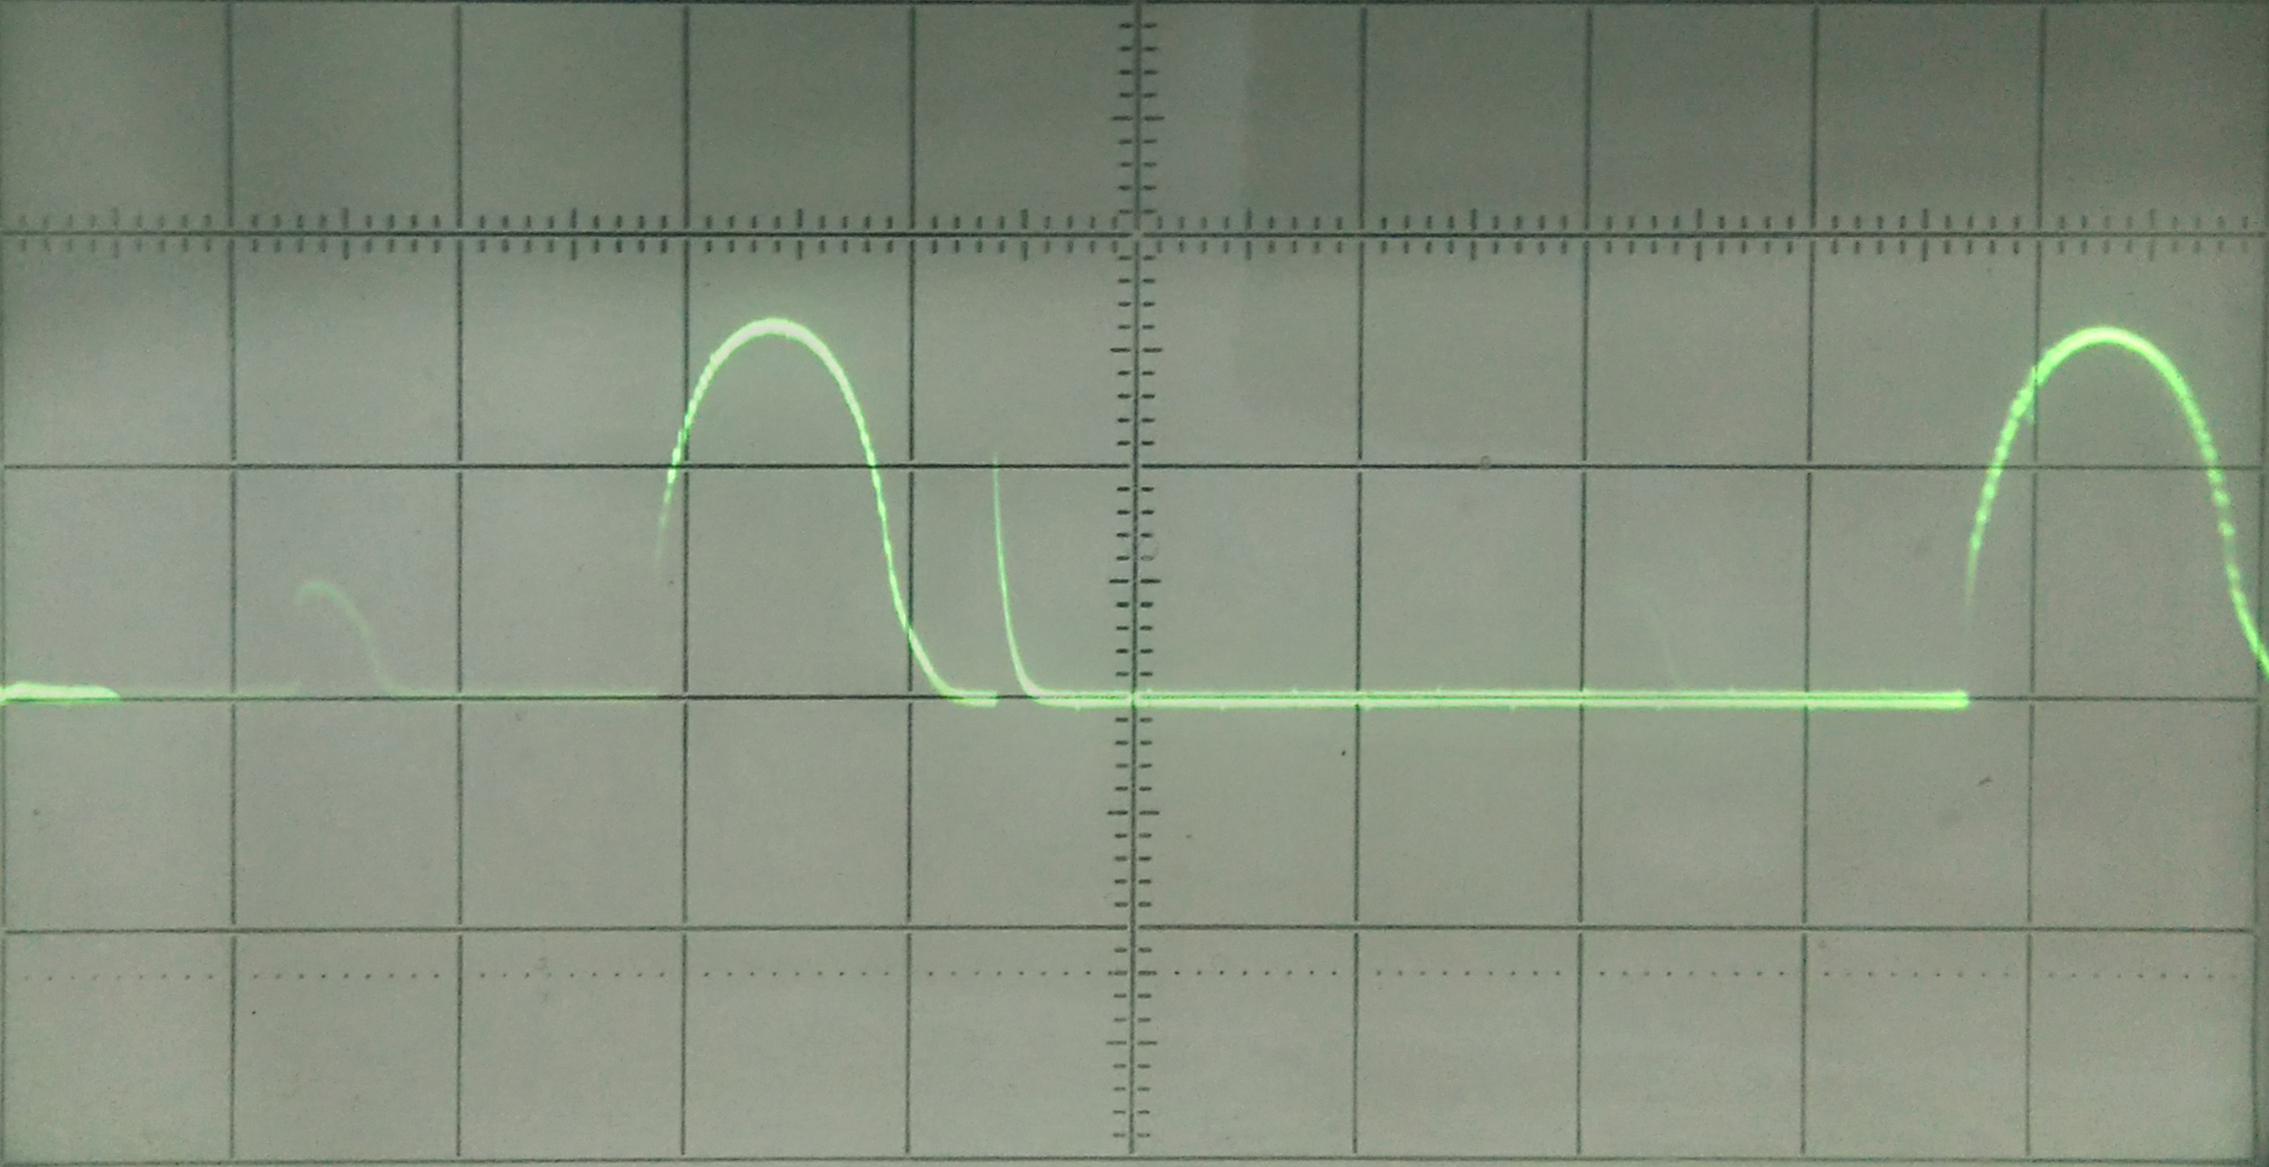
\includegraphics[width=\textwidth]{img/img11}}
		\caption{$U_{\text{отр}}=6$ В}
		\label{fig:img11}
	\end{minipage}
\end{figure}
На рис. \ref{fig:img2}-\ref{fig:img6}  и рис.\ref{fig:img7}-\ref{fig:img11} - показано, как меняются зоны при уменьшении $U_{\text{уск}}$ и $U_{\text{отр}}$ соответственно. 

%\newpage
Ширина частотной перестройки клистрона для трех зон генерации.

Для первой зоны она составила $\lambda_1=10.58-10.55=0.03$ см.

Для второй зоны -- $\lambda_2=10.6-10.515=0.085$ см.

Для третьей зоны -- $\lambda_3=10.58-10.515=0.065$ см.
\subsection{Задание 3 и 4}
% \subsubsection{Зависимость тока в цепи детектора от напряжения на отражателе}

% \begin{figure}[H]
% 		\centering
% 		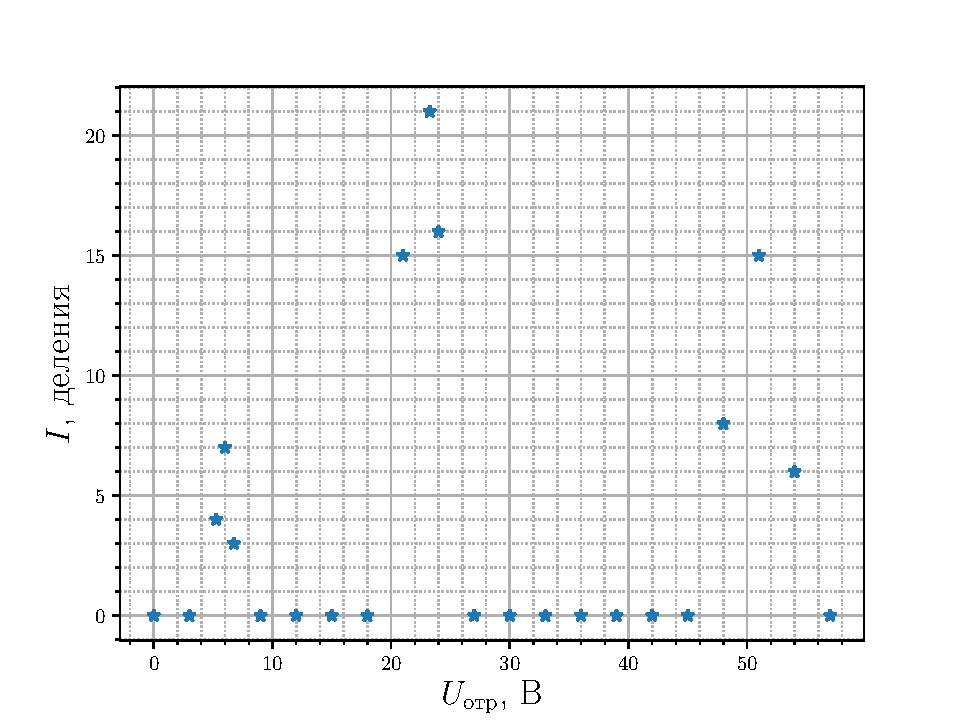
\includegraphics[height=0.4\textheight]{fig/res90V_1}
% 		\caption{$U_{\text{отр}}=90$ В}
% 		\label{fig:res90V_1}
% \end{figure}
% \begin{figure}[H]
% 		\centering
% 		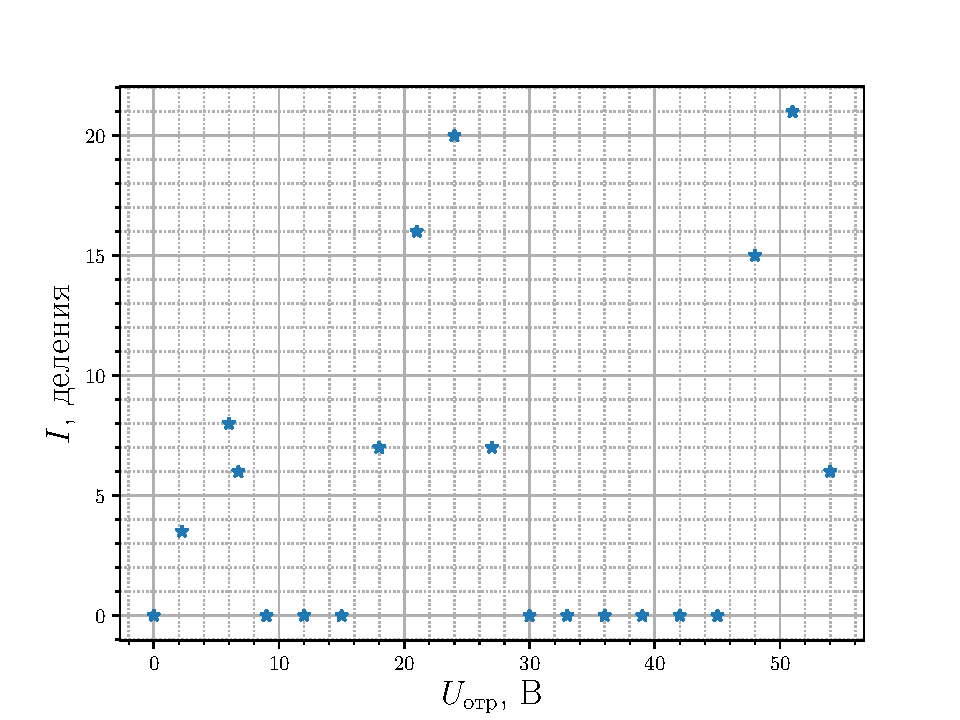
\includegraphics[height=0.4\textheight]{fig/res96V_1}
% 		\caption{$U_{\text{отр}}=96$ В}
% 		\label{fig:res96V_1}
% \end{figure}
% \begin{figure}[H]
% 		\centering
% 		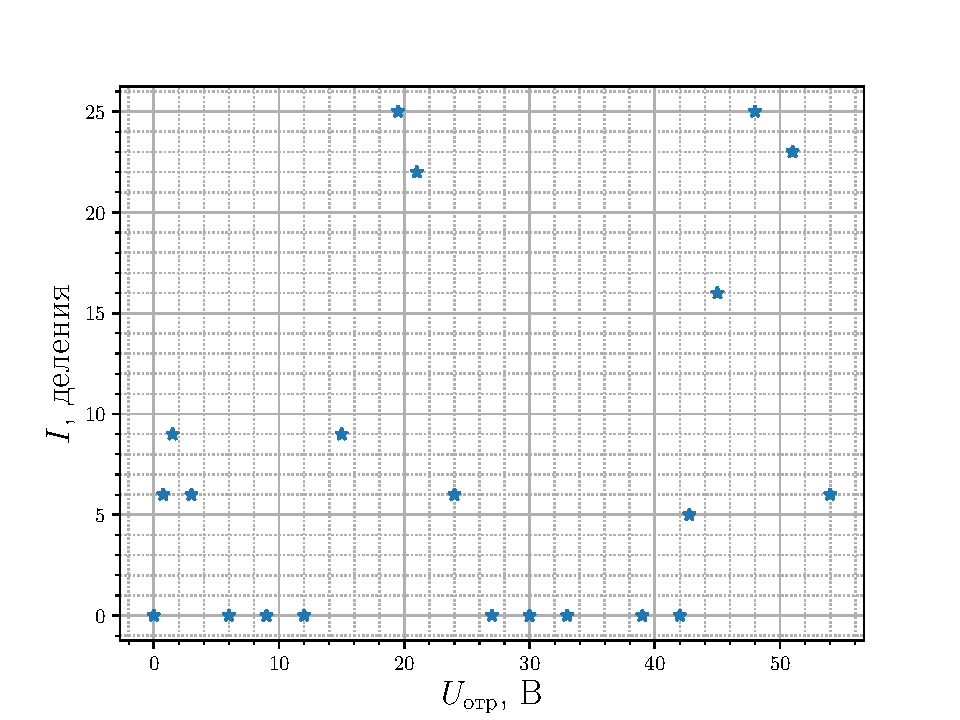
\includegraphics[height=0.4\textheight]{fig/res120V_1}
% 		\caption{$U_{\text{отр}}=120$ В}
% 		\label{fig:res120V_1}
% \end{figure}

\begin{figure}[H]
		\centering
		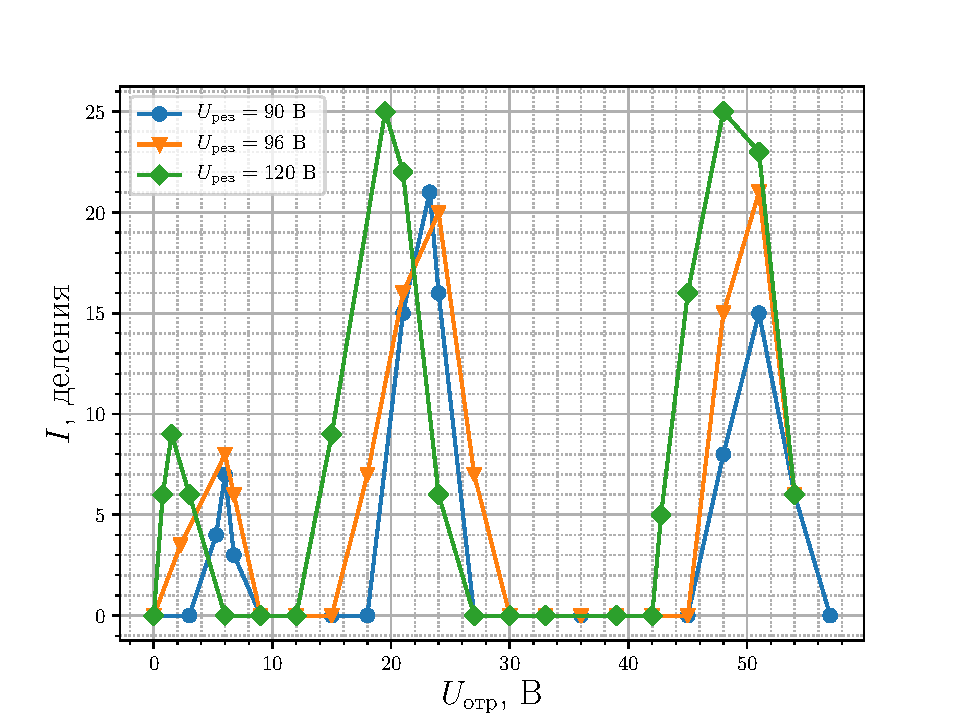
\includegraphics[width=\linewidth]{fig/task3a}
		\caption{Зависимость тока в цепи детектора от напряжения на отражателе}
		\label{fig:task3a}
\end{figure}
 
 Из графиков видно, что чем ниже номер зоны генерации, тем шире сама зона. В условии возбуждения клистрона величина $\theta _ { \text{г} }$ зависит от напряжения отражателя:

  $$\theta _ { \text{г} } = \frac { 2 m } { e } \frac { v _ { 0 } \omega L } { U _ { 0 } - U _ { \text{ oтр } } }.$$ 
  Здесь $U_{\text{отр}}<0$. Это значит, что чем больше по модулю $U_{\text{отр}}$, тем меньше $\theta _ { \text{г} }$ и больший диапазон $\theta _ { \text{г} }$ может убраться между $\pi+ 2\pi n$ и $2\pi(n+1)$.

\begin{figure}[H]
		\centering
		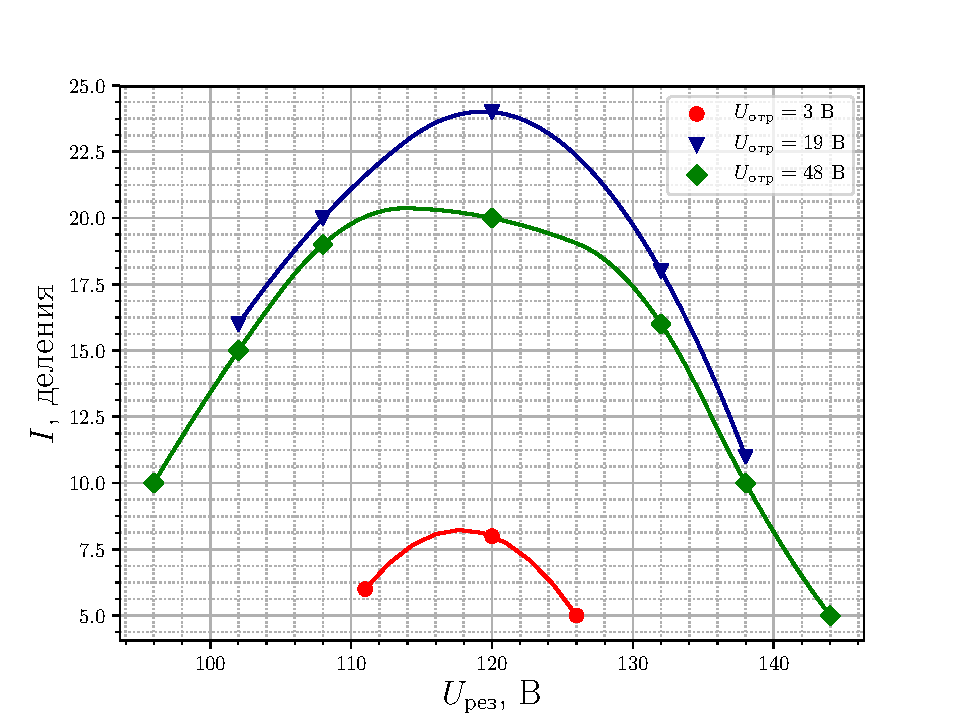
\includegraphics[width=\linewidth]{fig/task3b}
		\caption{Зависимость тока в цепи детектора от напряжения на отражателе}
		\label{fig:task3b}
\end{figure}


В центре каждой зоны генерации поток отдает резонатору наибольшую мощность $\displaystyle P_{max}\sim I_1 U_m \sim \frac{2I_0 XJ_1(X) U_0}{\theta _ { \text{г} }}$, где $J_1(X)$ - функция Бесселя первого порядка. Первая гармоника конвекционного тока достигает максимума при $X=1.84$. Следовательно, активная мощность, отдаваемая электронным потоком резонатору, достигает максимума в любой зоне генерации при $X=1.84$. Это, в частности, означает, что колебательное напряжение на зазоре $U_m$, соответствующее максимуму электронной мощности, возрастает с уменьшением номера зоны. В соответствии с выражением для максимальной мощности, с уменьшением номера зоны возрастают также и абсолютные значения максимумов электронной мощности. $$U_m=\frac{2U_0X}{M\theta _ { \text{г} }}=\frac{1.84 U_o}{\pi M(n+\frac 34)n}$$

%\newpage
% \subsubsection{Зависимость тока в цепи детектора от напряжения на резонаторе}
% \begin{figure}[H]
% 		\centering
% 		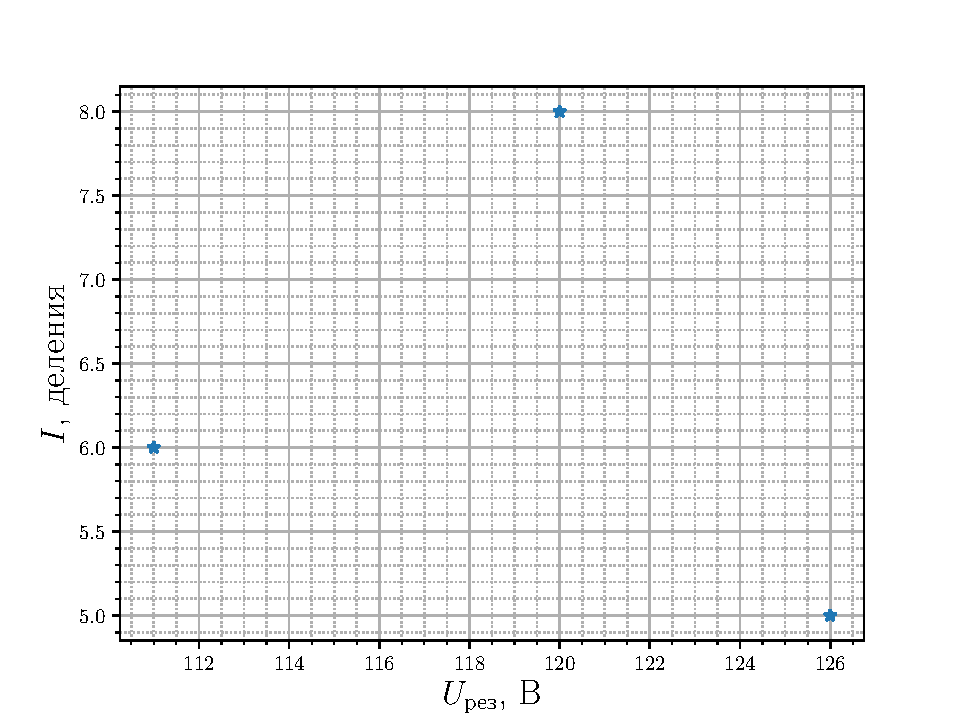
\includegraphics[height=0.4\textheight]{fig/ref3V_1}
% 		\caption{$U_{\text{рез}}=3$ В}
% 		\label{fig:ref3V_2}
% \end{figure}
% \begin{figure}[H]
% 		\centering
% 		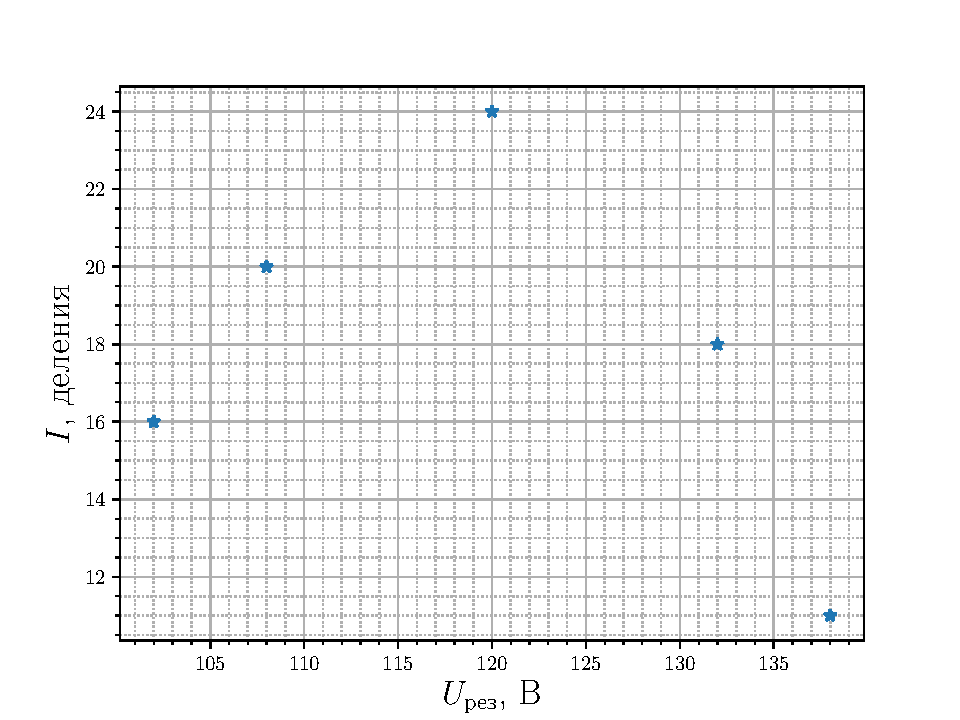
\includegraphics[height=0.4\textheight]{fig/ref19V_1}
% 		\caption{$U_{\text{рез}}=19$ В}
% 		\label{fig:ref19V_2}
% \end{figure}
% \begin{figure}[H]
% 		\centering
% 		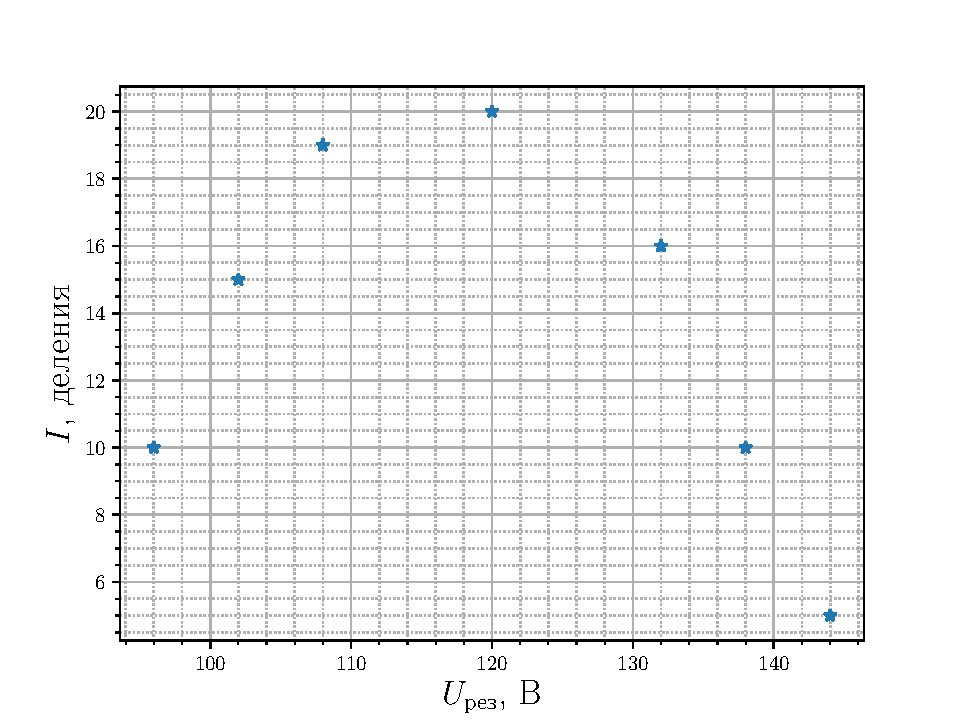
\includegraphics[height=0.4\textheight]{fig/ref48V_1}
% 		\caption{$U_{\text{рез}}=48$ В}
% 		\label{fig:ref48V_2}
% \end{figure}
\begin{figure}[H]
		\centering
		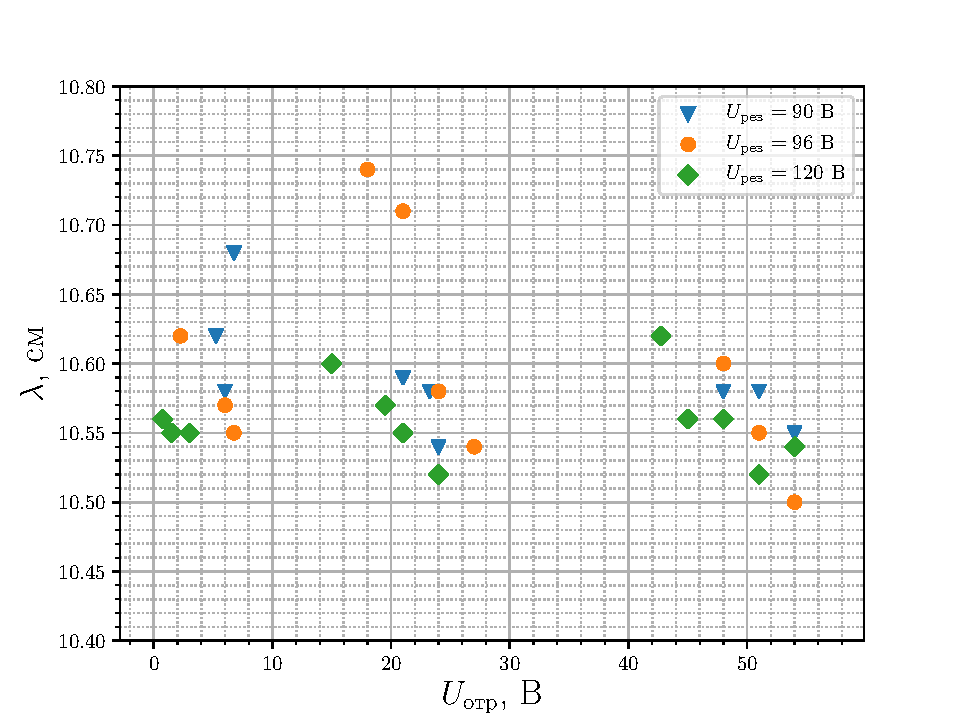
\includegraphics[width=\linewidth]{fig/task4a}
		\caption{Зависимость длины волны от напряжения на отражателе}
		\label{fig:task4a}
\end{figure}

При увеличении абсолютной величины $U_{\text{отр}}$ происходит рост частоты генерации клистрона. 

\begin{figure}[H]
		\centering
		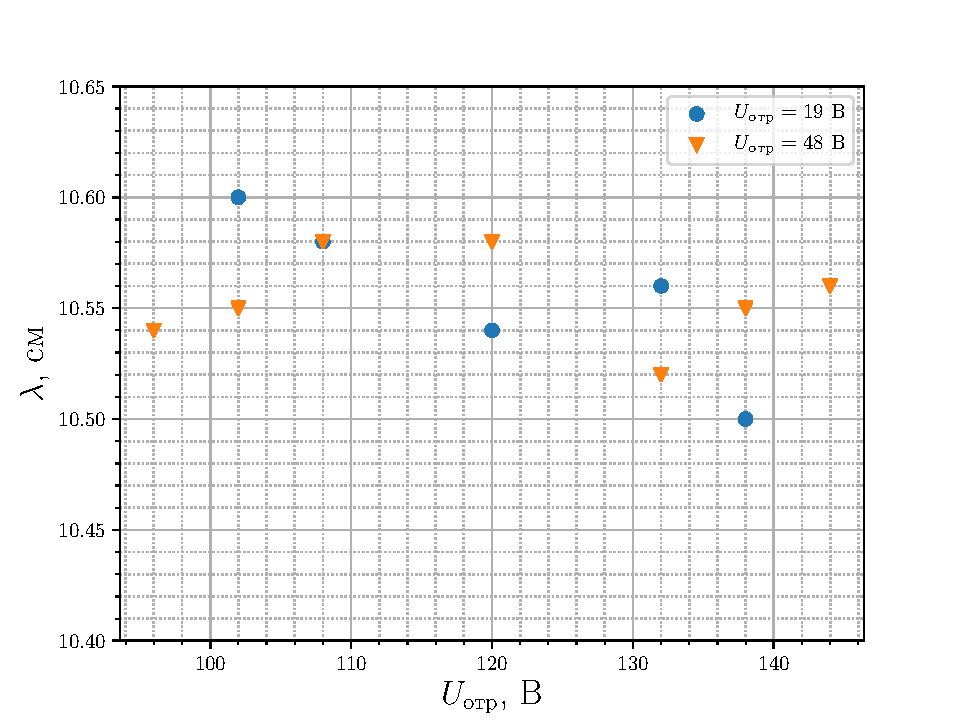
\includegraphics[width=\linewidth]{fig/task4b}
		\caption{Зависимость тока в цепи детектора от напряжения на резонаторе}
		\label{fig:task4b}
\end{figure}

% \subsection{Задание 4}
% %\newpage
% \subsubsection{Зависимость длины волны от напряжения на отражателе}

% \begin{figure}[H]
% 		\centering
% 		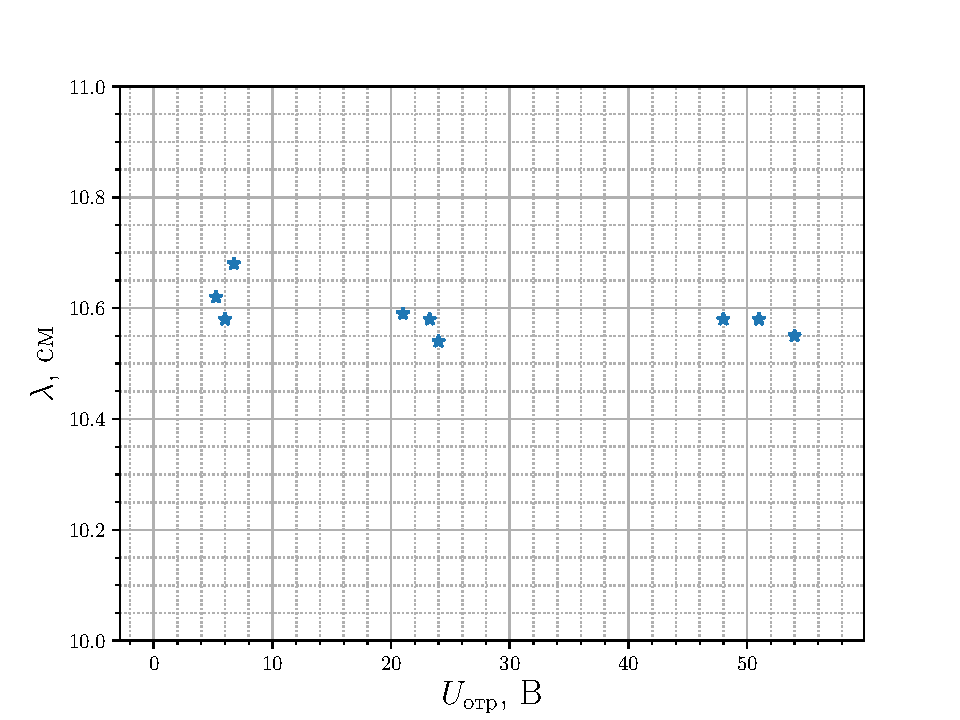
\includegraphics[height=0.4\textheight]{fig/res90V_2}
% 		\caption{$U_{\text{отр}}=90$ В}
% 		\label{fig:res90V_2}
% \end{figure}
% \begin{figure}[H]
% 		\centering
% 		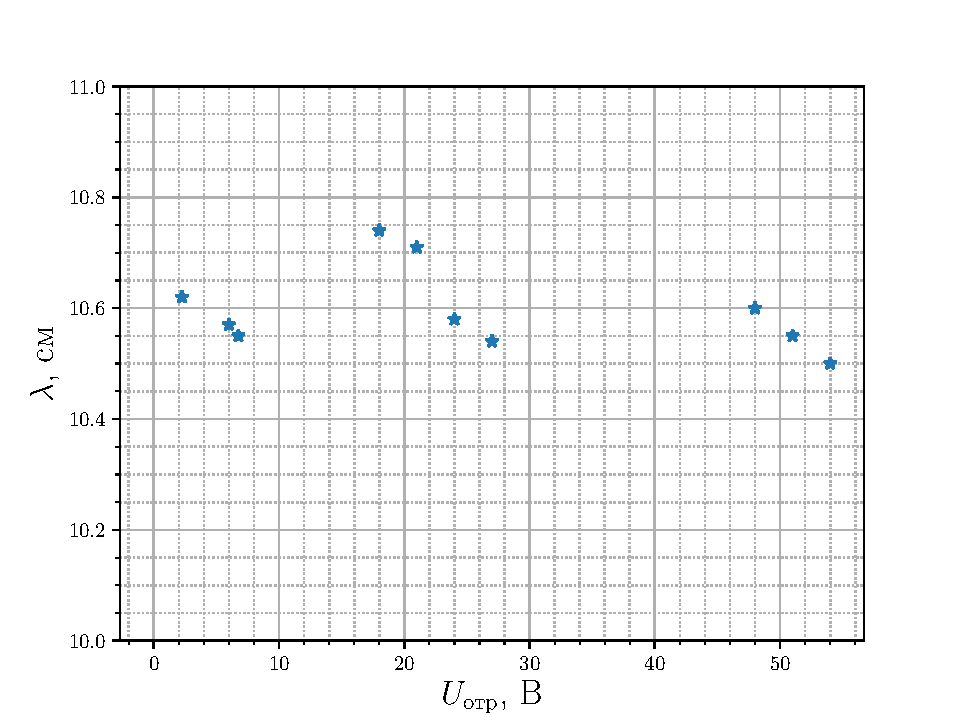
\includegraphics[height=0.4\textheight]{fig/res96V_2}
% 		\caption{$U_{\text{отр}}=96$ В}
% 		\label{fig:res96V_2}
% \end{figure}
% \begin{figure}[H]
% 		\centering
% 		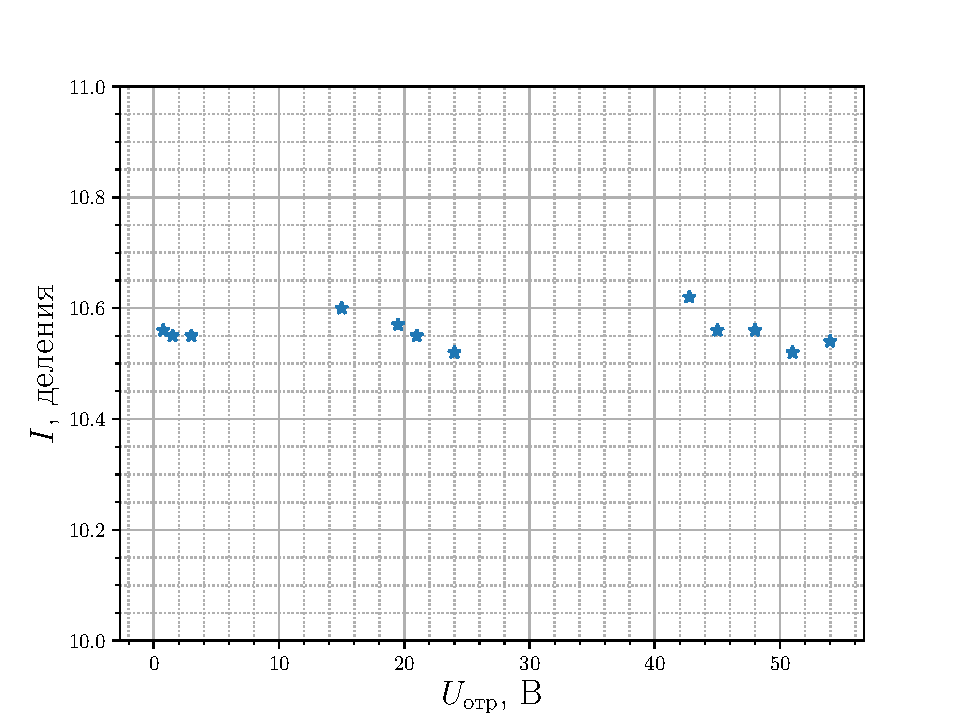
\includegraphics[height=0.4\textheight]{fig/res120V_2}
% 		\caption{$U_{\text{отр}}=120$ В}
% 		\label{fig:res120V_2}
% \end{figure}

%\newpage
% \subsubsection{Зависимость длины волны от напряжения на резонаторе}

% \begin{figure}[H]
% 		\centering
% 		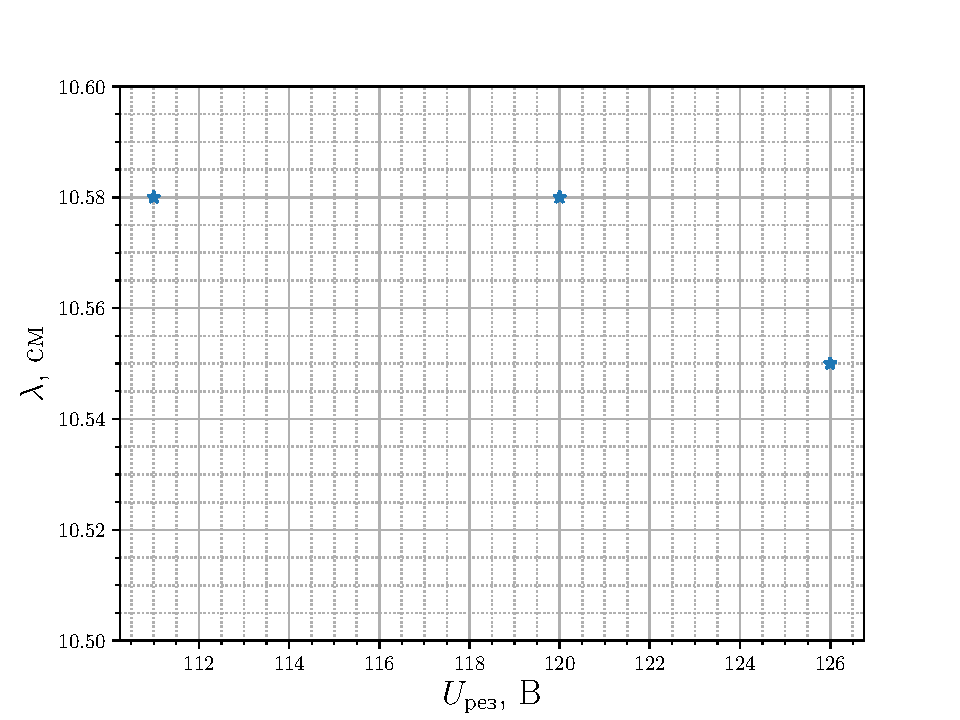
\includegraphics[height=0.4\textheight]{fig/ref3V_2}
% 		\caption{$U_{\text{рез}}=3$ В}
% 		\label{fig:ref3V_2}
% \end{figure}
% \begin{figure}[H]
% 		\centering
% 		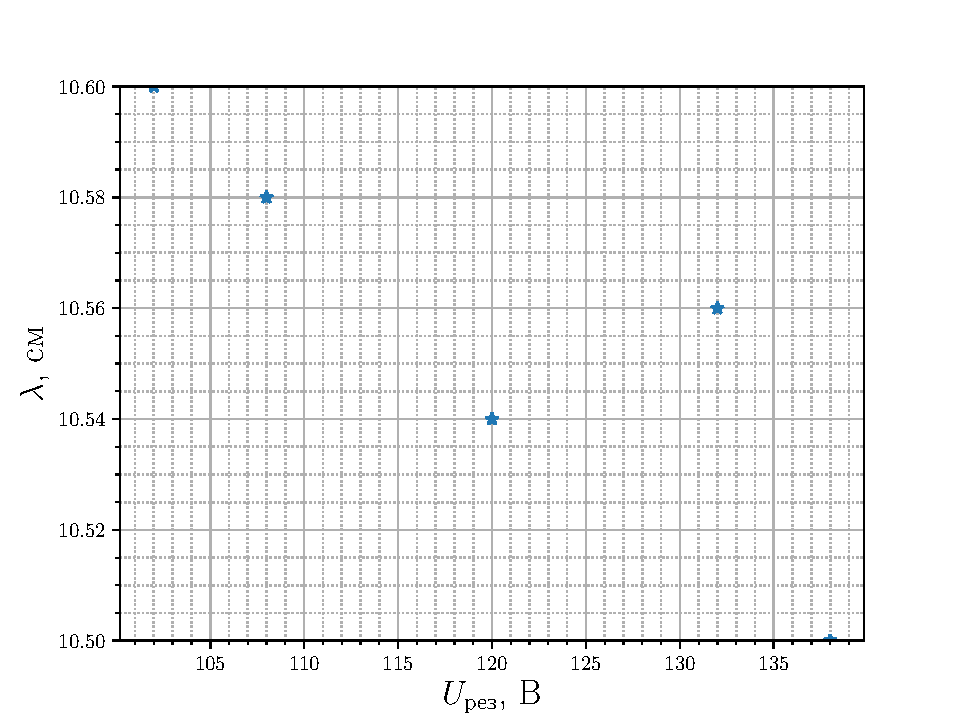
\includegraphics[height=0.4\textheight]{fig/ref19V_2}
% 		\caption{$U_{\text{рез}}=19$ В}
% 		\label{fig:ref19V_2}
% \end{figure}
% \begin{figure}[H]
% 		\centering
% 		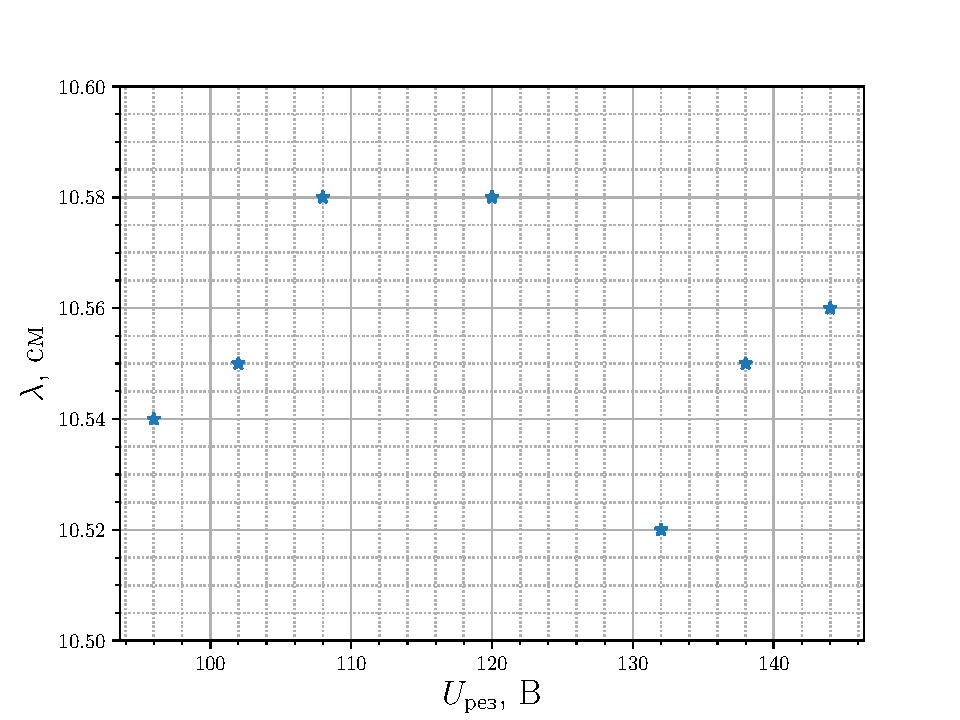
\includegraphics[height=0.4\textheight]{fig/ref48V_2}
% 		\caption{$U_{\text{рез}}=48$ В}
% 		\label{fig:ref48V_2}
% \end{figure}

%\newpage
\subsection{Задание 5}
% \begin{figure}[H]
% 		\centering
% 		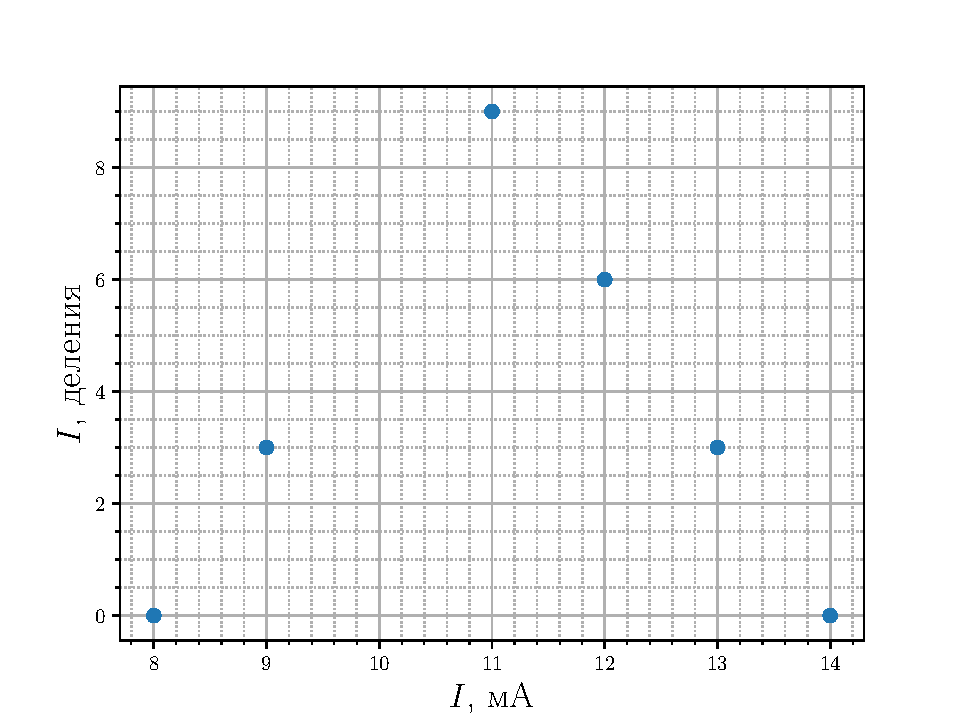
\includegraphics[height=0.4\textheight]{fig/res120Vref3V.pdf}
% 		\caption{$U_{\text{рез}}=120$ В, $U_{\text{отр}}=3$ В}
% 		\label{fig:res120Vref3V}
% \end{figure}
% \begin{figure}[H]
% 		\centering
% 		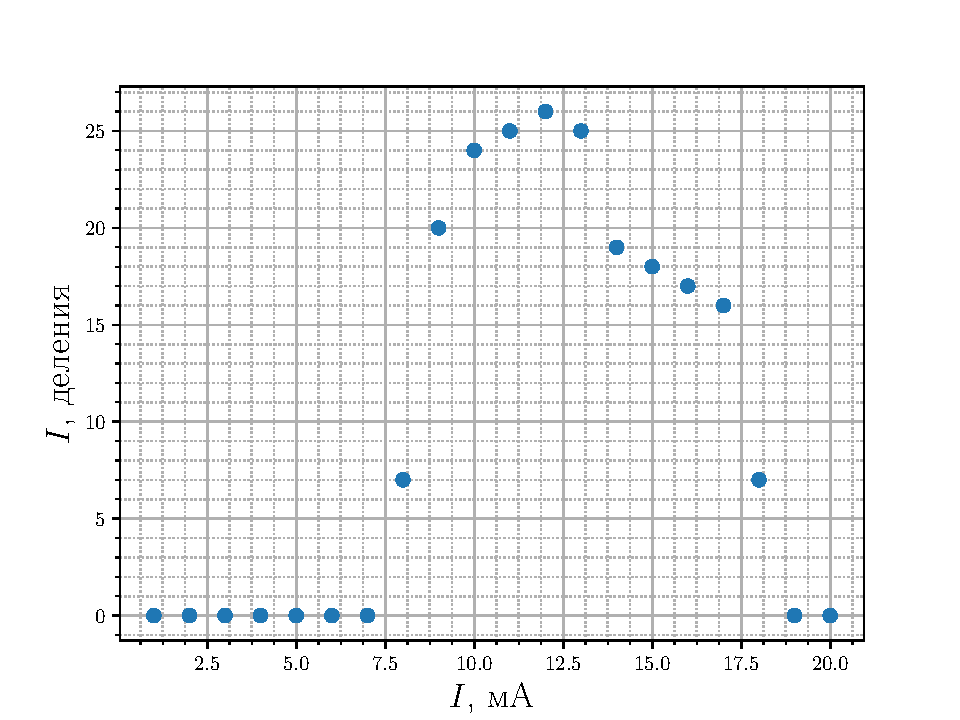
\includegraphics[height=0.4\textheight]{fig/res120Vref19V.pdf}
% 		\caption{$U_{\text{рез}}=120$ В, $U_{\text{отр}}=19$ В}
% 		\label{fig:res120Vref19V}
% \end{figure}
\begin{figure}[H]
		\centering
		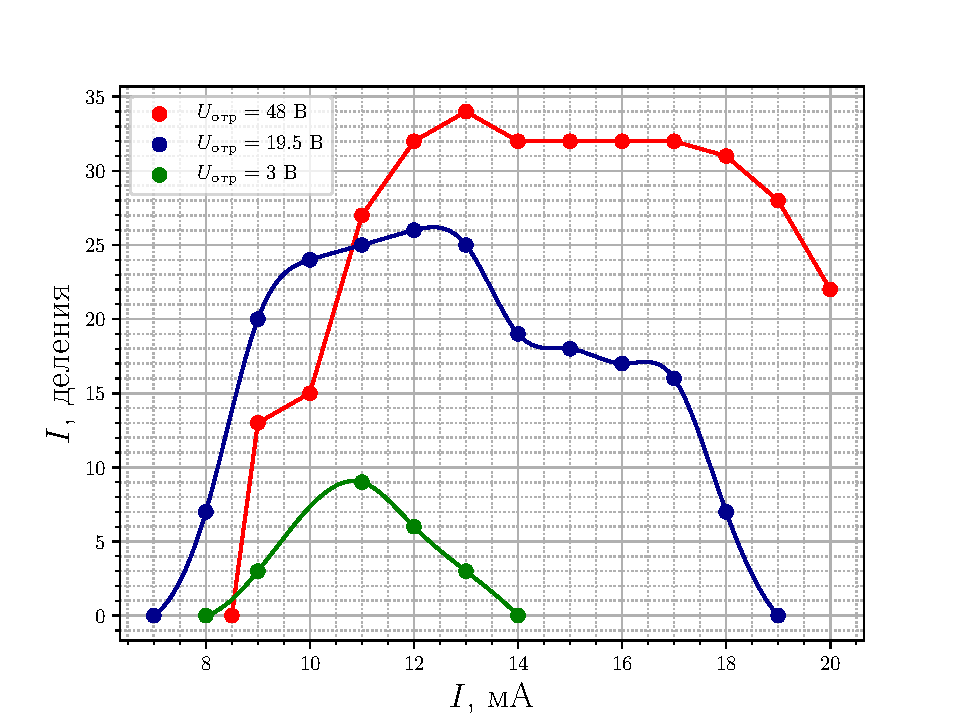
\includegraphics[height=0.4\textheight]{fig/task5}
		\caption{Зависимость тока в цепи детектора от тока пучка для трех различных зон генерации}
		\label{fig:task5}
\end{figure}

%\newpage

\section{Заключение}
В ходе работы было изучено устройство и основные принципы действия отражательного клистрона. Для математического описания использовалась теория тороидального резонатора, входящего в состав клистрона. Рассматривался процесс динамического управления плотностью в электронном пучке, возбуждение переменным конвекционным током пучка колебаний в резонаторе.  Рабочий режим соответствовал следующим напряжениям: 
\begin{itemize}
	\item $U_{\text{рез}}=96$ В
	\item $U_{\text{уск}}=126$ В
	\item $U_{\text{отр}}=42$ В
\end{itemize}

Получены зависимости тока в цепи детектора от напряжения на отражателе при постоянном напряжении на резонаторе и от напряжения на резонаторе при постоянном напряжении на отражателе. При помощи волномера измерена длина волны колебаний, создаваемых клистроном. А также, снята зависимость тока в цепи детектора от тока электронного пучка для трёх зон генератора. На основе экспериментальных данных были оценены ширина зазора в резонаторе и расстояние между резонатором и отражателем. Они получились равны соответственно 2 мм и 1 мм.
% \subsection{Контрольные вопросы}

% \begin{enumerate}
% 	\item Объясните принцип работы отражательного клистрона.
% 	\item Почему в приборах клистронного типа используются тороидальные ре­
% 	зонаторы?
% 	\item Можно ли для возвращения электронного потока в резонатор клистро­
% 	на использовать не постоянное электрическое, а постоянное магнитное поле?
% 	\item Что такое зоны генерации клистрона? Отличается ли структура поля
% 	в резонаторе для центров различных зон генерации?
% 	\item Как изменяется крутизна частотной перестройки клистрона с измене­
% 	нием номера зоны и при вариации добротности резонатора?
% \end{enumerate}

\begin{thebibliography}{}
	\bibitem{litlink1}  Гапонов В.И. Электроника. 4.11. М.: Физматгиз, 1960-
	\bibitem{litlink2}  Лебедев И.В. Техника и приборы СВЧ. Ч.Н. М.: Высшая школа, 1972.
	\bibitem{litlink3}  Коетиенко А.И. Введение в электронику СВЧ. М.: Изд. МГУ, 1989.
	\bibitem{litlink4}  Градштейн И.С., Рыжик Н.М. Таблицы интегралов, сумм рядов и про­
	изведений. М., 1963. 5
	\bibitem{litlink5}  Вайнштейн Л.А. Электромагнитные волны. М.: Радио и связь, 1988.
\end{thebibliography}
\end{document}